% My Dell XPS has aspect ratio 1610 (16:10).
% Screen settings of the presentation room are 16:9. 
% Supported options are 32, 43, 54, 141, 149, 169, 1610, 2013
\documentclass[aspectratio=169, c]{beamer}
% \includeonlyframes{current}


\usetheme{CambridgeUS}
\usecolortheme{dolphin}

% Alter template settings after loading it with \usetheme
\setbeamertemplate{navigation symbols}{}
\setbeamertemplate{itemize item}{$\blacktriangleright$}
\setbeamertemplate{itemize subitem}{$\triangleright$}

% Override footnote
\makeatletter
\setbeamertemplate{footline}{%
\leavevmode%
\hbox{%
    \begin{beamercolorbox}[wd=.2\paperwidth,ht=2.25ex,dp=1ex,center]{author in head/foot}%
        \usebeamerfont{author in head/foot} Software Science % \insertshortauthor\expandafter\beamer@ifempty\expandafter{\beamer@shortinstitute}{}{~~(\insertshortinstitute)}
    \end{beamercolorbox}%
    \begin{beamercolorbox}[wd=.6\paperwidth,ht=2.25ex,dp=1ex,center]{title in head/foot}%
        \usebeamerfont{title in head/foot}\insertshorttitle
    \end{beamercolorbox}%
    \begin{beamercolorbox}[wd=.2\paperwidth,ht=2.25ex,dp=1ex,right]{date in head/foot}%
        \usebeamerfont{date in head/foot}\insertshortdate{}\hspace*{2em}
        \textcolor{darkgray}{\insertframenumber{}} \hspace*{2ex} 
    \end{beamercolorbox}}%
    \vskip0pt%
}
\makeatother


% Load packages
\usepackage{amssymb}
\usepackage{amsmath}
\usepackage{bussproofs}
\usepackage{color,soul}
\makeatletter
\let\UL\ul
\renewcommand\ul{\let\set@color\beamerorig@set@color \let\reset@color\beamerorig@reset@color \UL}
\makeatother

\newcommand{\mypos}[2]{\tikz[remember picture,baseline=(#2.base)]{\node[inner sep=0pt, anchor=base](#2){#1};}}

\usepackage[style=authortitle]{biblatex}
\addbibresource{../thesis/bibliography.bib}
\DeclareFieldFormat{bibhypertarget}{#1}

\usepackage[perpage]{footmisc}
\renewcommand{\thefootnote}{\arabic{footnote}}  % Use numeric symbols for footnotes

\definecolor{ao}{rgb}{0.0, 0.5, 0.0}

\newcommand{\speechthis}[2]{
    \tikz[remember picture,baseline]{\node[anchor=base,inner sep=0,outer sep=0]%
    (#1) {\underline{#1}};\node[overlay,ellipse callout,fill=blue!50] 
    at ($(#1.north)+(-.5cm,0.8cm)$) {#2};}%
}%

\usepackage{tikz}
\usetikzlibrary{arrows.meta, calc, decorations.pathmorphing, decorations.pathreplacing, shapes.arrows,shapes.multipart,chains,patterns, quotes,tikzmark, trees, positioning}


\usepackage[newfloat]{minted}
\usepackage{mathtools}
\usepackage{marvosym}

\usepackage{pifont}

\usepackage{ulem}
\usepackage{varwidth}
\usepackage{wasysym}
\usepackage{xcolor}
\usepackage{xspace}

\usepackage{c-restrict-language}

% Custom commands
\def\eg{\textit{e.g.}\@\xspace}
\def\ie{\textit{i.e.}\@\xspace}
\def\etall{\textit{et al.}\@\xspace}

\def\cink{C-in-$\mathbb{K}\ $}
\def\cinkrestrict{\cink} %\textsubscript{restrict} 

\newcommand{\greentriangleright}[0]{\begingroup\color{green}\triangleright\endgroup}

\newcommand{\soutthick}[1]{%
    \renewcommand{\ULthickness}{1.4pt}%
       \sout{#1}%
    \renewcommand{\ULthickness}{.4pt}% Resetting to ulem default
}

\newcommand{\executionannotation}[2]{%
    {\centering
    \begin{minipage}{\textwidth}
    M:\\[4pt]
    \begin{tikzpicture}
    \node[rectangle,draw,align=left] (M) {#1};
    \end{tikzpicture}
    \end{minipage}

    \vspace*{5pt}

    \begin{minipage}{.37\textwidth}
    R:\\[4pt]
    #2
    \end{minipage}
    }
}

\newcommand{\cmark}{\ding{51}}%
\newcommand{\xmark}{\ding{55}}%

\setbeamerfont{footnote}{size=\tiny}

% Title page
\title{An operational semantics for the C99 restrict type qualifier}
\author{Ties Klappe}
\institute{Radboud University}
\date{May 7\textsuperscript{th} 2024}

\titlegraphic { 
\tikz[remember picture, overlay] {\node[anchor=south east] at (current page.south east)[yshift=\footheight] {\includegraphics[height=1.25cm]{ru-logo.png}};}
}

\begin{document}

\setlength{\fboxsep}{0pt}

% Render title page
\frame{\titlepage}

% Motivating example
% An example https://godbolt.org/z/h4rv6Y6G9
\begin{frame}[fragile]
\raggedright
\frametitle{A motivating example}

\begin{itemize}
    \item \textbf{Aliasing}: different symbolic names refer to the same object
    \item \textbf{Pointee}: the object pointed to by a pointer
\end{itemize}

\leavevmode\\

\begin{minted}[escapeinside=||,mathescape=true,linenos,texcomments]{c}
int foo1(int* p, int* q) {   
    *p = 10;
    *q = 11;
    return *p; // if $p$ and $q$ do not alias, $*p$ must evaluate to $10$
               // if $p$ and $q$ alias, $*p$ must evaluate to $11$
}
\end{minted}

\end{frame}

\begin{frame}[fragile]
\raggedright
\frametitle{A motivating example}

\begin{itemize}
    \item \textbf{Restrict}: programmer-provided information to inform the compiler specific pointers do not alias under certain conditions
\end{itemize}

\leavevmode \\

\begin{minted}[escapeinside=||,mathescape=true,linenos,texcomments]{c}
// \colorbox{blue!20}{Programmer}: hi compiler! I promise you $p$ and $q$ will not alias
int foo2(int* |\colorbox{blue!20}{restrict}| p, int* |\colorbox{blue!20}{restrict}| q) {
    *p = 10;
    *q = 11;
    return *p; // if $p$ and $q$ do not alias, $*p$ must evaluate to $10$
               // if $p$ and $q$ alias, $*p$ must evaluate to $11$
}
\end{minted}

\begin{figure}
\centering
\begin{tikzpicture}
    \node (p) {\mintinline{c}{p}};
    \node[right of = p, draw, rectangle] (pointee-p) {$10$};

    \node[right of = pointee-p] (q) {\mintinline{c}{q}};
    \node[right of = q, draw, rectangle] (pointee-q) {$11$};

    \draw[->] (p) -- (pointee-p);
    \draw[->] (q) -- (pointee-q);
\end{tikzpicture}
\end{figure}

\end{frame}


\begin{frame}[fragile]
\raggedright
\frametitle{A motivating example}
\begin{minted}[escapeinside=||,mathescape=true,linenos,texcomments]{c}
// \colorbox{blue!20}{Programmer}: hi compiler! I promise you $p$ and $q$ will not alias
// \colorbox{orange!20}{Compiler}: nice! Thanks to this information, I optimized your code
int foo2_optimized(int* |\colorbox{blue!20}{restrict}| p, int* |\colorbox{blue!20}{restrict}| q) {   
    *p = 10;
    *q = 11;
    return |\colorbox{orange!20}{\soutthick{*p} 10}|;
}

\end{minted}

\begin{figure}
\centering
\begin{tikzpicture}
    \node (p) {\mintinline{c}{p}};
    \node[right of = p, draw, rectangle] (pointee-p) {$10$};

    \node[right of = pointee-p] (q) {\mintinline{c}{q}};
    \node[right of = q, draw, rectangle] (pointee-q) {$11$};

    \draw[->] (p) -- (pointee-p);
    \draw[->] (q) -- (pointee-q);
\end{tikzpicture}
\end{figure}

\end{frame}

\begin{frame}[fragile]
\raggedright
\frametitle{The promise can be broken}
\begin{minipage}{0.4\textwidth}
\begin{minted}[escapeinside=||,mathescape=true,texcomments]{c}
int foo1(int* p, int* q) {   
    *p = 10;
    *q = 11;
    return *p;
}
\end{minted}
\end{minipage}%
\begin{minipage}{0.6\textwidth}
\begin{minted}[escapeinside=||,mathescape=true,texcomments]{c}
int foo2(int* |\colorbox{blue!20}{restrict}| p, int* |\colorbox{blue!20}{restrict}| q) {   
    *p = 10;
    *q = 11;
    return |\colorbox{orange!20}{\soutthick{*p} 10}|;
}
\end{minted}
\end{minipage}

\pause

\begin{minted}[escapeinside=||,mathescape=true,linenos,texcomments]{c}
int main() {
    int x;
    printf("%d, %d\n", foo1(&x, &x), foo2(&x, &x));
}
\end{minted}

\begin{figure}
\centering
\begin{tikzpicture}
    \node (p) {\mintinline{c}{p,q}};
    \node[right of = p, draw, rectangle, fill=red!20] (pointee) {$11$};

    \draw[->] (p) -- (pointee);
\end{tikzpicture}
\end{figure}

\begin{itemize}
    \item Prints $11, 10$, \ie the optimized code has a different result than the original code
    \item Is the optimization incorrect?
\end{itemize}

\end{frame}




\begin{frame}
\frametitle{Undefined behavior}
\begin{itemize}
    \item The programmer \textbf{broke} the promise by making $p$ and $q$ alias
    \item This induces \textbf{undefined behavior (UB, \rsub)}
    \begin{itemize}
        \item The compiler may \textit{assume} a program is free of UB
        \item It does not need to consider such programs when justifying optimizations (\ie the introductory optimization is sound)
    \end{itemize}
    \item In this presentation we only consider UB induced by restrict, but many other kinds exist
    (uninitialized memory loads, signed integer overflow, out-of-bounds accesses, ...)
\end{itemize}

\end{frame}

\begin{frame}
\frametitle{Undefined behavior}
\begin{itemize}
    \item To understand what uses of restrict induce undefined behavior, one should consult the ISO standard
\end{itemize}
\end{frame}

\begin{frame}
\frametitle{\textbf{6.7.3.1 Formal definition of} \texttt{restrict}}
\begin{figure}
\centering
{
\includegraphics[width=0.9\textwidth]{restrict-definition-1.png}
}
{
\\
\qquad \vdots
\\
}
{
\includegraphics[width=0.9\textwidth]{restrict-definition-3-4-annotation-defined.png}
}
{
\\
\qquad \vdots
}
\end{figure}
\end{frame}

\begin{frame}
    \frametitle{\textbf{6.7.3.1 Formal definition of} \texttt{restrict}}
\begin{minipage}{0.5\textwidth}
\begin{itemize}
    \item Four N-documents submitted since 2018
    \item \setulcolor{red}\ul{Gustedt (2024)}\footnotemark: ``By its title it is a promise (to provide a formal definition) but it is in fact very delicate mix up of semantic concepts that make it almost impossible to comprehend from the given text.'' 
    \item MacDonald \etall (2022, 2024)\footnotemark \ report a bug in the definition of ``based on''
\end{itemize}
\end{minipage}%
\begin{minipage}{0.5\textwidth}
\begin{figure}
\centering
{
\includegraphics[width=0.95\textwidth]{restrict-definition-1-annotated.png}
}
{
\\
\qquad \vdots
\\
}
{
\includegraphics[width=0.95\textwidth]{restrict-definition-3-4-annotated.png}
}
{
\\
\qquad \vdots
}
\end{figure}
\end{minipage}

\footnotetext[1]{\cite{semanticsgustedt2024}}
\footnotetext[2]{\cite{defectmacdonald2022}} 

\end{frame}

\begin{frame}
\frametitle{Goals}

We want a definition for restrict which is: \\
\begin{enumerate}
    \item \textbf{Unambiguous}, \ie a formal semantics
    \item \textbf{Consistent} with the standard definition (to the extent possible) and/or existing compiler optimizations
    \item \textbf{Executable} such that one can test a program for UB 
    \item \textbf{Suitable} to be used for proving compiler optimizations correct (future work)
\end{enumerate}

\end{frame}

\begin{frame}
\frametitle{Approach (formal semantics)}

% \footcite{leroy2016compcert}\footcite{krebbers2015c}\footcite{memarian2023cerberus}
\begin{itemize}
    \item A vast landscape of formal semantics exists for C, \eg CompCert, CH\textsubscript{2}O and Cerberus
    \item Most of these projects have omitted restrict, except the executable \cink semantics
\end{itemize}

\pause
\begin{itemize}
    \item The paper\footcite{hathhorn2015defining} contains only a single paragraph on restrict, an extensive evaluation reveals several problems (2)
    \item As a rewrite-based semantics, it is not suitable for reasoning about optimization correctness à la CompCert (4)
    \begin{figure}
        \centering
    
    \begin{enumerate}
        \item \textcolor{ao}{Unambiguous: \cmark}
        \item \textcolor{red!80}{Consistent: \xmark}
        \item \textcolor{ao}{Executable: \cmark}
        \item \textcolor{orange!80}{Suitable: \raisebox{-0.5ex}{\scalebox{1.3}{!}}}
    \end{enumerate}
\end{figure}
\end{itemize}


\end{frame}


\begin{frame}
\frametitle{Contributions}
\centering
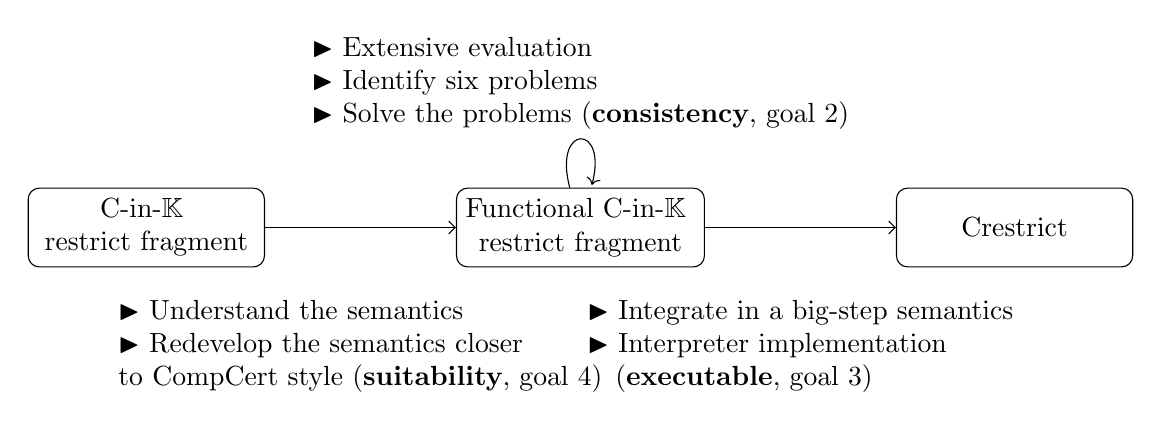
\begin{tikzpicture}[
    node distance=0.2\textwidth,
    artifact/.style={rectangle, rounded corners, minimum width=3cm, minimum height=1cm,text centered, draw=black,align=center}]

\node[artifact] (cink) {\cink\\restrict fragment};
\node[artifact, right = of cink] (cinkfunctional) {Functional \cink \\ restrict fragment};
\node[artifact, right = of cinkfunctional] (crestrict) {Crestrict};

\draw[-Straight Barb] (cink) -- (cinkfunctional)  node[midway, below=0.8cm, align=left] {%
    $\blacktriangleright$ Understand the semantics \\
    $\blacktriangleright$ Redevelop the semantics closer \\ to CompCert style (\textbf{suitability}, goal 4)
};

\path[-Straight Barb] (cinkfunctional) edge[loop above] node[midway, above, align=left] {%
    $\blacktriangleright$ Extensive evaluation \\ 
    $\blacktriangleright$ Identify six problems \\
    $\blacktriangleright$ Solve the problems (\textbf{consistency}, goal 2)
} (cinkfunctional);

\draw[-Straight Barb] (cinkfunctional) -- (crestrict) node[midway, right=1cm, below=0.8cm, align=left] {%
    $\blacktriangleright$ Integrate in a big-step semantics \\
    $\blacktriangleright$ Interpreter implementation \\ \quad (\textbf{executable}, goal 3)
};

\end{tikzpicture}
\end{frame}



% Restrict definition
\begin{frame}
\frametitle{Restrict definition (simplified)}
\begin{itemize}
    % \item A type qualifier for \textbf{pointer types}, \eg \mintinline{c}{int* restrict p;}
    \item A pointer is ``based on'' a restrict pointer if it depends on its value: \\
        \mintinline[mathescape=true]{c}{int x; int* restrict p = &x; int* q = p; // $q$ is based on $p$}  
    \item A \textbf{promise} that a restrict qualified pointer and pointers ``based on" it will \textbf{not alias} with other pointers during the \textbf{scope} it is alive if:
            \begin{itemize}
                \item The pointer is used to \textbf{access} the object it points to
                \item The object pointed to is \textbf{modified} (by any means)
            \end{itemize}
    % \item The compiler performs more optimizations based on this information
\end{itemize}
\end{frame}


% \begin{frame}
% \frametitle{The language\footnote{A small language based on \cite{blazy2009mechanized}}}
% \begin{figure}
% \[%\def\arraystretch{1.1}
% \begin{array}{lrl}
% \multicolumn{3}{l}{\hspace{-5pt}\textbf{Types}} \\[4pt]
% \textdom{st} \in \Simpletype                    & \bnfdef   & \Inttype \ | \ \Ptrtype  \ | \  \Arraytype \ | \ \Functiontype \ | \ \Voidtype  \\
%     \tau_q \in \Typequalifier                   & \bnfdef   & \Noqualifier \ | \ \Restrictqualifier \ | \ \Globalrestrictqualifier \\
%     \tau \in \Type                              & :=        & \Simpletype \times \Typequalifier       \\[4pt]
% \multicolumn{3}{l}{\hspace{-5pt}\textbf{Expressions and statements}} \\[4pt]
%     e \in \Expr                                 &   \bnfdef     & \Idvar \ | \ n \ | \ op_1  \ e \ | \ e_1 \ op_2 \ e_2 \ | \ \mathbin{*e} \ | \ \&e \ | \ ... \\
%     s \in \Statement                            &   \bnfdef     & e_1 = e_2 \ | \ e_1 = e_2(e^*) \ | \ e(e^*) \ | \ s_1; s_2 \ | \ \mathsf{if}(e) \ s_1 \ \mathsf{else} \ s_2 \ | \\
%                                                 &               & ...
% \end{array}
% \]
% \end{figure}

% \end{frame}

% \begin{frame}
% \frametitle{The language\footnote{A small language based on \cite{blazy2009mechanized}}}
% \begin{figure}
% \[%\def\arraystretch{1.1}
% \begin{array}{lrl}
% \multicolumn{3}{l}{\hspace{-5pt}\textbf{Types}} \\[4pt]
% \textdom{st} \in \Simpletype                    & \bnfdef   & \Inttype \ | \ \Ptrtype  \ | \ \text{\soutthick{\Arraytype}} \ | \ \text{\soutthick{\Functiontype}} \ | \ \text{\soutthick{\Voidtype}}  \\
%     \tau_q \in \Typequalifier                   & \bnfdef   & \Noqualifier \ | \ \Restrictqualifier \ | \ \text{\soutthick{\Globalrestrictqualifier}} \\
%     \tau \in \Type                              & :=        & \Simpletype \times \Typequalifier       \\[4pt]
% \multicolumn{3}{l}{\hspace{-5pt}\textbf{Expressions and statements}} \\[4pt]
%     e \in \Expr                                 &   \bnfdef     & \Idvar \ | \ n \ | \ op_1  \ e \ | \ e_1 \ op_2 \ e_2 \ | \ \mathbin{*e} \ | \ \&e \ | \ ... \\
%     s \in \Statement                            &   \bnfdef     & e_1 = e_2 \ | \ e_1 = e_2(e^*) \ | \ e(e^*) \ | \ s_1; s_2 \ | \ \mathsf{if}(e) \ s_1 \ \mathsf{else} \ s_2 \ | \\
%                                                 &               & ...
% \end{array}
% \]
% \end{figure}

% \end{frame}

\begin{frame}
\frametitle{The language\footnote{A small language based on \cite{blazy2009mechanized}} (simplified)}
\begin{figure}
\[%\def\arraystretch{1.1}
\begin{array}{lrl}
\multicolumn{3}{l}{\hspace{-5pt}\textbf{Types}} \\[4pt]
\textdom{st} \in \Simpletype                    & \bnfdef   & \Inttype \ | \ \mathsf{Ptr} \ \colorbox{blue!20}{$\tau$}  \\
    \tau_q \in \Typequalifier                   & \bnfdef   & \Noqualifier \ | \ \colorbox{blue!20}{\Restrictqualifier} \\
    \tau \in \Type                              & \bnfdef   & (\textdom{st}, \tau_q) %\Simpletype \times \Typequalifier       \\[4pt]
% \multicolumn{3}{l}{\hspace{-5pt}\textbf{Expressions and statements}} \\[4pt]
%     e \in \Expr                                 &   \bnfdef     & \Idvar \ | \ n \ | \ op_1  \ e \ | \ e_1 \ op_2 \ e_2 \ | \ \mathbin{*e} \ | \ \&e \ | \ ... \\
%     s \in \Statement                            &   \bnfdef     & e_1 = e_2 \ | \ e_1 = e_2(e^*) \ | \ e(e^*) \ | \ s_1; s_2 \ | \ \mathsf{if}(e) \ s_1 \ \mathsf{else} \ s_2 \ | \\
%                                                 &               & ...
\end{array}
\]
\end{figure}

\end{frame}

\begin{frame}[fragile]
\frametitle{The \cinkrestrict semantics}
Two features are jointly used to support restrict:\\
\begin{enumerate}
    \item Pointer values have some extra information, called \textbf{\textcolor{blue}{bases}}
    \begin{itemize}
        \item Tracks on which restrict qualified pointer(s) a pointer is based
        \item Used to distinguish pointers to the same address
    \end{itemize}
    \vspace*{5pt}
    \[
    \begin{array}{lll}
    \Blockvar \in \Block, \Scopeidvar \in \Scopeid &  :=  & \Intdomain \\
    \Basesvar \in \Bases & := & \Set{\mypos{$\Block$}{cink-provenance-block} \times \mypos{$\Scopeid$}{cink-provenance-scope}} \\~\\
    \strut\Val  & \bnfdef   & \ptr{(\mypos{$\Block$}{cink-abstract-val} \times \textcolor{blue}{\Bases})} \ | \ ... 
    \end{array}
    \hspace{1000pt minus 1fill}
    \]

\pause

    \begin{tikzpicture}[overlay, remember picture]
    \draw[red!30] ([yshift=-2pt]cink-abstract-val.base east)--([yshift=-2pt]cink-abstract-val.base west) to[bend left=25] ++(-.75,-.25) node[red!60, anchor=east] {\footnotesize Address of the pointee};
    \draw[blue!30] ([yshift=-2pt]cink-provenance-block.base east)--([yshift=-2pt]cink-provenance-block.base west) to[bend left=25] ++(-.75, -.25) node[blue!60, anchor=east] {\footnotesize Address of restrict pointer};
    \draw[blue!30] ([yshift=-2pt]cink-provenance-scope.base west)--([yshift=-2pt]cink-provenance-scope.base east) to[bend right=25] ++(.75, -.25) node[blue!60, anchor=west] {\footnotesize Restrict pointer declaration scope};
    
    \end{tikzpicture}
\end{enumerate}

\end{frame}

\begin{frame}[fragile]
    \frametitle{The \cinkrestrict semantics}
    Two features are jointly used to support restrict:\\
    \begin{enumerate}
        \setcounter{enumi}{1}
        \item The \textbf{restrict stack} tracks what memory accesses are allowed by maintaining a per-location \textbf{restrict state}
    \end{enumerate}

    \[
    \begin{array}{lll}
    \Restrictstate  &   \bnfdef     & \mypos{$\onlyread{\Basesvar}$}{cink-stack-or} \ | \ \mypos{$\restricted{\Basesvar}$}{cink-stack-rs} \ | \ \mypos{$\unrestricted$}{cink-stack-un} \\~\\
    R \in \Restrictstack  & := & \List{\mypos{$\Scopeid$}{cink-stack-scope} \times (\Block \rightarrow \Restrictstate)}
    \end{array}
    \hspace{1000pt minus 1fill}
    \]

\pause

    \begin{tikzpicture}[overlay, remember picture]
    \draw[red!30] ([yshift=-2pt]cink-stack-or.base east)--([yshift=-2pt]cink-stack-or.base west) to[bend left=25] ++(-.75,-.25) node[red!60, align=left, anchor=east, yshift=-5pt] {\footnotesize Load via \ptr{(\_, \Basesvar)}};
    \draw[red!30] ([yshift=-2pt]cink-stack-rs.base east)--([yshift=-2pt]cink-stack-rs.base west) to[bend left=25] ++(-.5,-.25) node[red!60, align=left, anchor=center,yshift=-5pt] {\footnotesize Store via \ptr{(\_, \Basesvar)}};
    \draw[red!30] ([yshift=-2pt]cink-stack-un.base east)--([yshift=-2pt]cink-stack-un.base west) to[bend right=25] ++(.5,-.25) node[red!60, align=left, anchor=west,yshift=-5pt] {\footnotesize Loads via pointers with different bases};
    \draw[red!30] ([yshift=-2pt]cink-stack-scope.base west)--([yshift=-2pt]cink-stack-scope.base east) to[bend right=25] ++(.75,-.25) node[red!60, align=left, anchor=west] {\footnotesize Scope in which the access occured};
    \end{tikzpicture}

\end{frame}

\begin{frame}[fragile]
\frametitle{The introductory example under the \cinkrestrict semantics}
\begin{minted}[escapeinside=||,mathescape=true,texcomments]{c}
// Scope \scope{foo}
int foo(int* restrict p, int* restrict q) {   
    *p = 10;
    *q = 11;
    return *p;
}
\end{minted}

\begin{figure}[h]
\centering
\begin{minipage}{.33\textwidth}
\begin{minted}[escapeinside=||,mathescape=true,texcomments]{c}
// Scope \scope{main}
|\colorbox{red!20}{int main() \{}|
    int x;
    foo(&x, &x);
}
\end{minted}
\end{minipage}%
\begin{minipage}{.67\textwidth}
\executionannotation
{
    $\emptyset$
}
{
    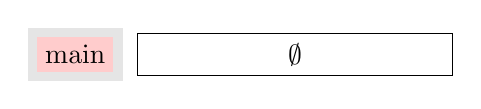
\begin{tikzpicture}[stack/.style={rectangle split, rectangle split parts=#1, draw, anchor=center, text centered},
        scope/.style={fill=gray!20, anchor=center}]
    \node[stack=1, minimum width=4.0cm] (s) {
    \nodepart{one} $\emptyset$
    };
    \node[scope, left=5pt of s.one west]   {\colorbox{red!20}{\scope{main}}};
    \end{tikzpicture}   
}
\end{minipage}
\end{figure}

\end{frame}


% ----

\begin{frame}[fragile]
\frametitle{The introductory example under the \cinkrestrict semantics}
\begin{minted}[escapeinside=||,mathescape=true,texcomments]{c}
// Scope \scope{foo}
int foo(int* restrict p, int* restrict q) {   
    *p = 10;
    *q = 11;
    return *p;
}
\end{minted}

\begin{figure}[h]
\centering
\begin{minipage}{.33\textwidth}
\begin{minted}[escapeinside=||,mathescape=true,texcomments]{c}
// Scope \scope{main}
int main() {
    |\colorbox{red!20}{int x;}| // $\&x = \Blockvar_x$
    foo(&x, &x);
}
\end{minted}
\end{minipage}%
\begin{minipage}{.67\textwidth}
\executionannotation
{
\{\colorbox{red!20}{$\Blockvar_x \mapsto \vundef$}\}
}
{
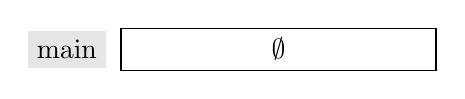
\begin{tikzpicture}[stack/.style={rectangle split, rectangle split parts=#1, draw, anchor=center, text centered},
        scope/.style={fill=gray!20, anchor=center}]
\node[stack=1, minimum width=4.0cm] (s) {
\nodepart{one} $\emptyset$
};
\node[scope, left=5pt of s.one west]   {\scope{main}};

\end{tikzpicture}
}
\end{minipage}
\end{figure}

\end{frame}


% ----

\begin{frame}[fragile]
\frametitle{The introductory example under the \cinkrestrict semantics}
\begin{minted}[escapeinside=||,mathescape=true,texcomments]{c}
// Scope \scope{foo} \quad $\&p = \Blockvar_p$ \quad $\&q = \Blockvar_q$
int foo(int* restrict p, int* restrict q) { 
    *p = 10;
    *q = 11;
    return *p;
}
\end{minted}

\begin{figure}[h]
\centering
\begin{minipage}{.33\textwidth}
\begin{minted}[escapeinside=||,mathescape=true,texcomments]{c}
// Scope \scope{main}
int main() {
    int x; // $\&x = \Blockvar_x$
    |\colorbox{red!20}{foo(&x, &x);}|
}
\end{minted}
\end{minipage}%
\begin{minipage}{.67\textwidth}
\executionannotation
{
\{\colorbox{red!20}{$\Blockvar_p \mapsto \ptr{(\Blockvar_x, \set{(\Blockvar_p, \scope{foo})})}$},\\
                                            \ \colorbox{red!20}{$\Blockvar_q \mapsto \ptr{(\Blockvar_x, \set{(\Blockvar_q, \scope{foo})})}$}, \\
                                            \ $\Blockvar_x \mapsto \vundef$\}
}
{
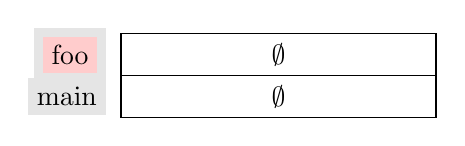
\begin{tikzpicture}[stack/.style={rectangle split, rectangle split parts=#1, draw, anchor=center, text centered},
        scope/.style={fill=gray!20, anchor=center}]
\node[stack=2, minimum width=4.0cm] (s) {
    \nodepart{one} $\emptyset$
    \nodepart{two} $\emptyset$
};
\node[scope, left=5pt of s.one west]   {\colorbox{red!20}{\scope{foo}}};
\node[scope, left=5pt of s.two west]   {\scope{main}};

\end{tikzpicture}
}
\end{minipage}
\end{figure}
\end{frame}

% ----

\begin{frame}[fragile]
\frametitle{The introductory example under the \cinkrestrict semantics}
\begin{minted}[escapeinside=||,mathescape=true,texcomments]{c}
// Scope \scope{foo} \quad $\&p = \Blockvar_p$ \quad $\&q = \Blockvar_q$
int foo(int* restrict p, int* restrict q) {   
    |\colorbox{red!20}{*p = 10;}|
    *q = 11;
    return *p;
}
\end{minted}

\begin{figure}[h]
\centering
\begin{minipage}{.33\textwidth}
\begin{minted}[escapeinside=||,mathescape=true,texcomments]{c}
// Scope \scope{main}
int main() {
    int x; // $\&x = \Blockvar_x$
    foo(&x, &x);
}
\end{minted}
\end{minipage}%
\begin{minipage}{.67\textwidth}
\executionannotation
{\{$\Blockvar_p \mapsto \ptr{(\Blockvar_x, \set{(\Blockvar_p, \scope{foo})})}$,\\
                                            \ $\Blockvar_q \mapsto \ptr{(\Blockvar_x, \set{(\Blockvar_q, \scope{foo})})}$, \\
                                            \ $\Blockvar_x \mapsto \colorbox{red!20}{10}$\}
}
{
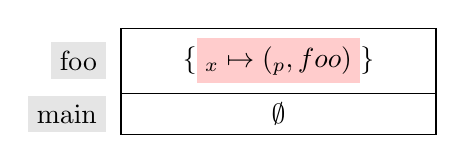
\begin{tikzpicture}[stack/.style={rectangle split, rectangle split parts=#1, draw, anchor=center, text centered},
        scope/.style={fill=gray!20, anchor=center}]
% Stack
\node[stack=2, minimum width=4.0cm] (s) {
    \nodepart{one} \{\colorbox{red!20}{$\Blockvar_x \mapsto \restricted{\set{(\Blockvar_p, \scope{foo})}}$}\}
    \nodepart{two} $\emptyset$
};

% Scopes
\node[scope, left=5pt of s.one west]   {\scope{foo}};
\node[scope, left=5pt of s.two west]   {\scope{main}};

\end{tikzpicture}
}
\end{minipage}
\end{figure}

\end{frame}


% ----

\begin{frame}[fragile]
\frametitle{The introductory example under the \cinkrestrict semantics}
\begin{minted}[escapeinside=||,mathescape=true,texcomments]{c}
// Scope \scope{foo} \quad $\&p = \Blockvar_p$ \quad $\&q = \Blockvar_q$
int foo(int* restrict p, int* restrict q) {   
    *p = 10;
    |\colorbox{red!20}{*q = 11;}|
    return *p;
}
\end{minted}
\vspace*{-30pt}
\begin{figure}[h]
\centering
\begin{minipage}{.33\textwidth}
\begin{minted}[escapeinside=||,mathescape=true,texcomments]{c}
// Scope \scope{main}
int main() {
    int x; // $\&x = \Blockvar_x$
    foo(&x, &x);
}
\end{minted}
\end{minipage}%
\begin{minipage}{.67\textwidth}
\colorbox{red!20}{$\restricted{\set{(\Blockvar_\text{\textcolor{blue}{$q$}}, \scope{foo})}} \joinsym \restricted{\set{(\Blockvar_\text{\textcolor{blue}{$p$}}, \scope{foo})}} = ...$}
\\

\executionannotation
{\{$\Blockvar_p \mapsto \ptr{(\Blockvar_x, \set{(\Blockvar_p, \scope{foo})})}$,\\
                                            \ $\Blockvar_q \mapsto \ptr{(\Blockvar_x, \set{(\Blockvar_q, \scope{foo})})}$, \\
                                            \ $\Blockvar_x \mapsto \vundef$\}
}
{
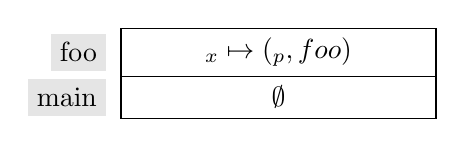
\begin{tikzpicture}[stack/.style={rectangle split, rectangle split parts=#1, draw, anchor=center, text centered},
        scope/.style={fill=gray!20, anchor=center}]
% Stack
\node[stack=2, minimum width=4.0cm] (s) {
    \nodepart{one} $\set{\Blockvar_x \mapsto \restricted{\set{(\Blockvar_p, \scope{foo})}}}$
    \nodepart{two} $\emptyset$
};

% Scopes
\node[scope, left=5pt of s.one west]   {\scope{foo}};
\node[scope, left=5pt of s.two west]   {\scope{main}};

\end{tikzpicture}
}
\end{minipage}
\end{figure}

\end{frame}




% ----

\begin{frame}[fragile]
\frametitle{The introductory example under the \cinkrestrict semantics}
\colorbox{red!20}{$\restricted{\set{(\Blockvar_\text{\textcolor{blue}{$q$}}, \scope{foo})}} \joinsym \restricted{\set{(\Blockvar_\text{\textcolor{blue}{$p$}}, \scope{foo})}} = ...$}

\begin{minipage}{.5\textwidth}
\begin{itemize}
    \item The symmetric \joinsym \ operation describes the result of joining two restrict states \\~\\
    \item \footnotesize$\unresabbr = \unrestricted$, $\resabbr{\Basesvar} = (\restricted{\Basesvar})$ and $\orabbr{\Basesvar} = (\onlyread{\Basesvar})$
    \item \footnotesize$\Basesvar \neq \Basesvar'$
\end{itemize}
\end{minipage}%
\begin{minipage}{.5\textwidth}

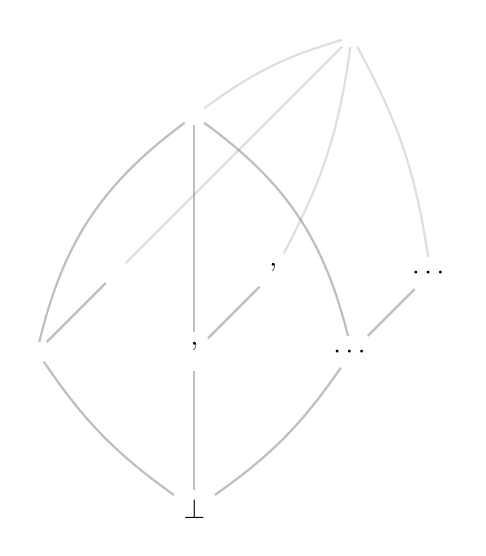
\begin{tikzpicture}
    \node (ub)     at (7,5) {\rsub};
    \node (un)     at (5,4) {\unresabbr};
    \node (rsbs)   at (4,2) {\resabbr{\Basesvar}};
    \node (rsbs')  at (6,2) {\resabbr{\Basesvar'}};
    \node (rsbs'') at (8,2) {$\cdots$};
    \node (orbs)   at (3,1) {\orabbr{\Basesvar}};
    \node (orbs')  at (5,1) {\orabbr{\Basesvar'}};
    \node (orbs'') at (7,1) {$\cdots$};
    \node (bot)    at (5,-1) {$\bot$};

    \path[thick, black, opacity=0.25]
    (bot) edge[bend left=10] node {} (orbs)
    (bot) edge node {} (orbs')
    (bot) edge[bend right=10] node {} (orbs'')
    
    (orbs) edge node {} (rsbs) 
    (orbs') edge node {} (rsbs')
    (orbs'') edge node {} (rsbs'')  
    
    (orbs) edge[bend left=20] node {} (un)
    (orbs') edge node {} (un)
    (orbs'') edge[bend right=20] node {} (un)

    (rsbs) edge[gray] node {} (ub)
    (rsbs') edge[bend right=10, gray] node {} (ub)
    (rsbs'') edge[bend right=10, gray] node {} (ub)

    (un) edge[bend left=10, gray] node {} (ub);
\end{tikzpicture}
\end{minipage}

\end{frame}


% ----

\begin{frame}[fragile]
\frametitle{The introductory example under the \cinkrestrict semantics}

\colorbox{red!20}{$\restricted{\set{(\Blockvar_\text{\textcolor{blue}{$q$}}, \scope{foo})}} \joinsym \restricted{\set{(\Blockvar_\text{\textcolor{blue}{$p$}}, \scope{foo})}} = \rsub$}

\begin{minipage}{.5\textwidth}
\begin{itemize}
    \item The symmetric \joinsym \ operation describes the result of joining two restrict states \\~\\
    \item \footnotesize$\unresabbr = \unrestricted$, $\resabbr{\Basesvar} = (\restricted{\Basesvar})$ and $\orabbr{\Basesvar} = (\onlyread{\Basesvar})$
    \item \footnotesize$\Basesvar \neq \Basesvar'$
\end{itemize}
\end{minipage}%
\begin{minipage}{.5\textwidth}

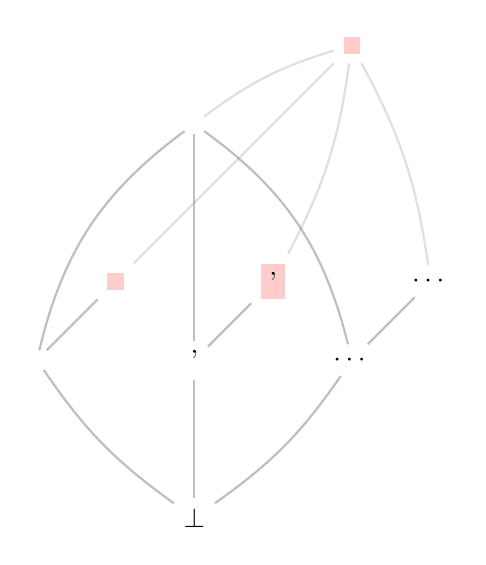
\begin{tikzpicture}
    \node (ub)     at (7,5) {\colorbox{red!20}{\rsub}};
    \node (un)     at (5,4) {\unresabbr};
    \node (rsbs)   at (4,2) {\colorbox{red!20}{\resabbr{\Basesvar}}};
    \node (rsbs')  at (6,2) {\colorbox{red!20}{\resabbr{\Basesvar'}}};
    \node (rsbs'') at (8,2) {$\cdots$};
    \node (orbs)   at (3,1) {\orabbr{\Basesvar}};
    \node (orbs')  at (5,1) {\orabbr{\Basesvar'}};
    \node (orbs'') at (7,1) {$\cdots$};
    \node (bot)    at (5,-1) {$\bot$};

    \path[thick, black, opacity=0.25]
    (bot) edge[bend left=10] node {} (orbs)
    (bot) edge node {} (orbs')
    (bot) edge[bend right=10] node {} (orbs'')
    
    (orbs) edge node {} (rsbs) 
    (orbs') edge node {} (rsbs')
    (orbs'') edge node {} (rsbs'')  
    
    (orbs) edge[bend left=20] node {} (un)
    (orbs') edge node {} (un)
    (orbs'') edge[bend right=20] node {} (un)

    (rsbs) edge[gray] node {} (ub)
    (rsbs') edge[bend right=10, gray] node {} (ub)
    (rsbs'') edge[bend right=10, gray] node {} (ub)

    (un) edge[bend left=10, gray] node {} (ub);
\end{tikzpicture}
\end{minipage}

\end{frame}

% ----

\begin{frame}[fragile]
\frametitle{The introductory example under the \cinkrestrict semantics}
\begin{minted}[escapeinside=||,mathescape=true,texcomments]{c}
// Scope \scope{foo} \quad $\&p = \Blockvar_p$ \quad $\&q = \Blockvar_q$
int foo(int* restrict p, int* restrict q) {   
    *p = 10;
    |\colorbox{red!20}{*q = 11;}|
    return *p;
}
\end{minted}
\vspace*{-30pt}
\begin{figure}[h]
\centering
\begin{minipage}{.33\textwidth}
\begin{minted}[escapeinside=||,mathescape=true,texcomments]{c}
// Scope \scope{main}
int main() {
    int x; // $\&x = \Blockvar_x$
    foo(&x, &x);
}
\end{minted}
\end{minipage}%
\begin{minipage}{.67\textwidth}
\textbf{UB}: \colorbox{red!20}{$\restricted{\set{(\Blockvar_\text{\textcolor{blue}{$q$}}, \scope{foo})}} \joinsym \restricted{\set{(\Blockvar_\text{\textcolor{blue}{$p$}}, \scope{foo})}} = \rsub$}
\\

\executionannotation
{\{$\Blockvar_p \mapsto \ptr{(\Blockvar_x, \set{(\Blockvar_p, \scope{foo})})}$,\\
                                            \ $\Blockvar_q \mapsto \ptr{(\Blockvar_x, \set{(\Blockvar_q, \scope{foo})})}$, \\
                                            \ $\Blockvar_x \mapsto \vundef$\}
}
{
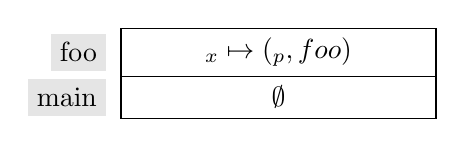
\begin{tikzpicture}[stack/.style={rectangle split, rectangle split parts=#1, draw, anchor=center, text centered},
        scope/.style={fill=gray!20, anchor=center}]
% Stack
\node[stack=2, minimum width=4.0cm] (s) {
    \nodepart{one} $\set{\Blockvar_x \mapsto \restricted{\set{(\Blockvar_p, \scope{foo})}}}$
    \nodepart{two} $\emptyset$
};

% Scopes
\node[scope, left=5pt of s.one west]   {\scope{foo}};
\node[scope, left=5pt of s.two west]   {\scope{main}};

\end{tikzpicture}
}
\end{minipage}
\end{figure}

\end{frame}



\begin{frame}
\frametitle{Evaluating the \cinkrestrict semantics}
\begin{itemize}
\item The semantics correctly gives undefined behavior to our introductory example! \\ \ But, we argue, there are some problems: \\
\item Too much undefined behavior (TMU)
    \begin{itemize}
        \item \colorbox{ao!20}{Aliasing loads}
        \item Returning restrict pointers
    \end{itemize}
\item Too little undefined behavior (TLU)
    \begin{itemize}
        \item Array of restrict pointers
        \item Nested restrict pointers
        \item Semantic preservation under inlining
        \item Call to free  
    \end{itemize}
\end{itemize}

\end{frame}

\begin{frame}[fragile]
\frametitle{Aliasing loads (TMU)}
\begin{minipage}{0.7\textwidth}
\begin{minted}[escapeinside=||,mathescape=true,linenos]{c}
// Scope $\scope{h}$
void h(int* q, int* restrict r, int* restrict s) {
    *q = *r + *s; 
}
// Scope $\scope{main}$
int main() {
    int x, y;
    int* restrict p = &y;
    *p = 0; 
    h(&x, p, p);
}
\end{minted}
\end{minipage}%
\begin{minipage}[t]{0.3\textwidth}
\begin{tikzpicture}
    \node (q) {\mintinline{c}{q}};
    \node[right of = q] (pointee-q) {$x$};

    \node[right of = pointee-p] (rs) {\mintinline{c}{r,s}};
    \node[right of = rs] (pointee-rs) {$y$};

    \draw[->] (q) -- (pointee-q);
    \draw[->] (rs) -- (pointee-rs);
\end{tikzpicture}
\end{minipage}

\begin{itemize}
    \item Simplified version of example 3 from the ISO standard demonstrating DB
    \item $y$ does \textbf{not} get \textbf{modified} in the scope \scope{h} of \mintinline{c}{r,s}
\end{itemize}

\end{frame}


% ----


\begin{frame}[fragile]
\frametitle{Aliasing loads (TMU)}
\begin{minted}[escapeinside=||,mathescape=true]{c}
// Scope $\scope{h}$
void h(int* q, int* restrict r, int* restrict s) {
    *q = *r + *s; 
}
\end{minted}

\begin{figure}[h]
\centering
\begin{minipage}{.36\textwidth}
\begin{minted}[escapeinside=||,mathescape=true]{c}
// Scope $\scope{main}$
|\colorbox{red!20}{int main() \{}|
    int x, y;
    int* restrict p = &y;
    *p = 0; 
    h(&x, p, p);
}
\end{minted}
\end{minipage}%
\begin{minipage}{.674\textwidth}
\executionannotation
{
    $\emptyset$
}
{
    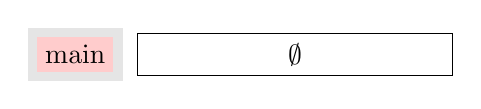
\begin{tikzpicture}[stack/.style={rectangle split, rectangle split parts=#1, draw, anchor=center, text centered},
        scope/.style={fill=gray!20, anchor=center}]
    \node[stack=1, minimum width=4.0cm] (s) {
    \nodepart{one} $\emptyset$
    };
    \node[scope, left=5pt of s.one west]   {\colorbox{red!20}{\scope{main}}};
    \end{tikzpicture}   
}
\end{minipage}
\end{figure}

\end{frame}


% ----


\begin{frame}[fragile]
\frametitle{Aliasing loads (TMU)}
\begin{minted}[escapeinside=||,mathescape=true]{c}
// Scope $\scope{h}$
void h(int* q, int* restrict r, int* restrict s) {
    *q = *r + *s; 
}
\end{minted}

\begin{figure}[h]
\centering
\begin{minipage}{.36\textwidth}
\begin{minted}[escapeinside=||,mathescape=true]{c}
// Scope $\scope{main}$
int main() {
    |\colorbox{red!20}{int x, y;}|
    int* restrict p = &y;
    *p = 0; 
    h(&x, p, p);
}
\end{minted}
\end{minipage}%
\begin{minipage}{.64\textwidth}
\executionannotation
{
\{\colorbox{red!20}{$\Blockvar_x \mapsto \vundef, \Blockvar_y \mapsto \vundef$}\}
}
{
    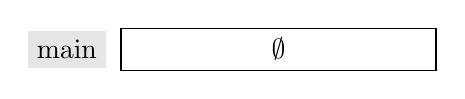
\begin{tikzpicture}[stack/.style={rectangle split, rectangle split parts=#1, draw, anchor=center, text centered},
        scope/.style={fill=gray!20, anchor=center}]
    \node[stack=1, minimum width=4.0cm] (s) {
    \nodepart{one} $\emptyset$
    };
    \node[scope, left=5pt of s.one west]   {\scope{main}};
    \end{tikzpicture}   
}
\end{minipage}
\end{figure}

\end{frame}


% ---- 


\begin{frame}[fragile]
\frametitle{Aliasing loads (TMU)}
\begin{minted}[escapeinside=||,mathescape=true]{c}
// Scope $\scope{h}$
void h(int* q, int* restrict r, int* restrict s) {
    *q = *r + *s; 
}
\end{minted}

\begin{figure}[h]
\centering
\begin{minipage}{.36\textwidth}
\begin{minted}[escapeinside=||,mathescape=true]{c}
// Scope $\scope{main}$
int main() {
    int x, y;
    |\colorbox{red!20}{int* restrict p = &y;}|
    *p = 0;
    h(&x, p, p);
}
\end{minted}
\end{minipage}%
\begin{minipage}{.64\textwidth}
\executionannotation
{
\{$\Blockvar_x \mapsto \vundef$, \\
    \ $\Blockvar_y \mapsto \vundef$, \\
    \ \colorbox{red!20}{$\Blockvar_p \mapsto \ptr{(\Blockvar_y, \set{(\Blockvar_p, \scope{main})})}$}
\}
}
{
    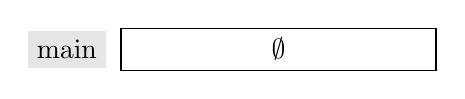
\begin{tikzpicture}[stack/.style={rectangle split, rectangle split parts=#1, draw, anchor=center, text centered},
        scope/.style={fill=gray!20, anchor=center}]
    \node[stack=1, minimum width=4.0cm] (s) {
    \nodepart{one} $\emptyset$
    };
    \node[scope, left=5pt of s.one west]   {\scope{main}};
    \end{tikzpicture}   
}
\end{minipage}
\end{figure}


\end{frame}


% ---- 


\begin{frame}[fragile]
\frametitle{Aliasing loads (TMU)}
\begin{minted}[escapeinside=||,mathescape=true]{c}
// Scope $\scope{h}$
void h(int* q, int* restrict r, int* restrict s) {
    *q = *r + *s; 
}
\end{minted}

\begin{figure}[h]
\centering
\begin{minipage}{.36\textwidth}
\begin{minted}[escapeinside=||,mathescape=true]{c}
// Scope $\scope{main}$
int main() {
    int x, y;
    int* restrict p = &y;
    |\colorbox{red!20}{*p = 0;}|
    h(&x, p, p);
}
\end{minted}
\end{minipage}%
\begin{minipage}{.64\textwidth}
\executionannotation
{
\{$\Blockvar_x \mapsto \vundef$, \\
    \ $\Blockvar_y \mapsto \colorbox{red!20}{0}$, \\
    \ $\Blockvar_p \mapsto \ptr{(\Blockvar_y, \set{(\Blockvar_p, \scope{main})})}$
\}
}
{
    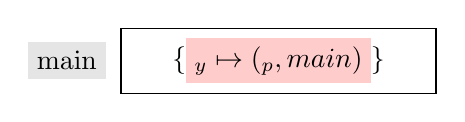
\begin{tikzpicture}[stack/.style={rectangle split, rectangle split parts=#1, draw, anchor=center, text centered},
        scope/.style={fill=gray!20, anchor=center}]
    \node[stack=1, minimum width=4.0cm] (s) {
    \nodepart{one} \{\colorbox{red!20}{$\Blockvar_y \mapsto \restricted{\set{(\Blockvar_p, \scope{main})}}$}\}
    };
    \node[scope, left=5pt of s.one west]   {\scope{main}};
    \end{tikzpicture}   
}
\end{minipage}
\end{figure}


\end{frame}


% ---- 


\begin{frame}[fragile]
\frametitle{Aliasing loads (TMU)}
\begin{minted}[escapeinside=||,mathescape=true]{c}
// Scope $\scope{h}$
void h(int* q, int* restrict r, int* restrict s) {
    *q = *r + *s; 
}
\end{minted}
\vspace*{-1cm}
\begin{figure}[h]
\centering
\begin{minipage}{.36\textwidth}
\begin{minted}[escapeinside=||,mathescape=true]{c}
// Scope $\scope{main}$
int main() {
    int x, y;
    int* restrict p = &y;
    *p = 0;
    |\colorbox{red!20}{h(&x, p, p);}|
}
\end{minted}
\end{minipage}%
\begin{minipage}{.64\textwidth}
\executionannotation
{
\{$\Blockvar_x \mapsto \vundef$, $\Blockvar_y \mapsto 0$, \\
    \ $\Blockvar_p \mapsto \ptr{(\Blockvar_y, \set{(\Blockvar_p, \scope{main})})}$, \\
    \ \colorbox{red!20}{$\Blockvar_q \mapsto \ptr{(\Blockvar_x, \emptyset)}$}, \\
    \ \colorbox{red!20}{$\Blockvar_r \mapsto \ptr{(\Blockvar_y, \set{(\Blockvar_r, \scope{h}), (\Blockvar_p, \scope{main})})} $}, \\
    \ \colorbox{red!20}{$\Blockvar_s \mapsto \ptr{(\Blockvar_y, \set{(\Blockvar_s, \scope{h}), (\Blockvar_p, \scope{main})})} $} \\
\}
}
{
    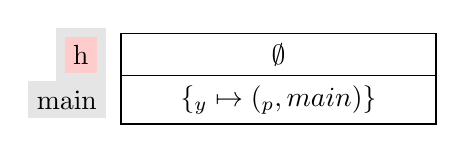
\begin{tikzpicture}[stack/.style={rectangle split, rectangle split parts=#1, draw, anchor=center, text centered},
        scope/.style={fill=gray!20, anchor=center}]
    \node[stack=2, minimum width=4.0cm] (s) {
    \nodepart{one} $\emptyset$
    \nodepart{two} \{$\Blockvar_y \mapsto \restricted{\set{(\Blockvar_p, \scope{main})}}$\}
    };
    \node[scope, left=5pt of s.one west]   {\colorbox{red!20}{\scope{h}}};
    \node[scope, left=5pt of s.two west]   {\scope{main}};
    \end{tikzpicture}   
}
\end{minipage}
\end{figure}

\end{frame}



% ---- 


\begin{frame}[fragile]
\frametitle{Aliasing loads (TMU)}
\begin{minted}[escapeinside=||,mathescape=true]{c}
// Scope $\scope{h}$
void h(int* q, int* restrict r, int* restrict s) {
    *q = |\colorbox{red!20}{*r}| + *s; 
}
\end{minted}
\vspace*{-1cm}
\begin{figure}[!h]
\begin{minipage}[t]{.36\textwidth}

\begin{minted}[escapeinside=||,mathescape=true]{c}
// Scope $\scope{main}$
int main() {
    int x, y;
    int* restrict p = &y;
    *p = 0;
    h(&x, p, p);
}
\end{minted}
\end{minipage}%
\begin{minipage}{.64\textwidth}
\executionannotation
{
\{$\Blockvar_x \mapsto \vundef$, $\Blockvar_y \mapsto 0$, \\
    \ $\Blockvar_p \mapsto \ptr{(\Blockvar_y, \set{(\Blockvar_p, \scope{main})})}$, \\
    \ $\Blockvar_q \mapsto \ptr{(\Blockvar_x, \emptyset)}$, \\
    \ $\Blockvar_r \mapsto \ptr{(\Blockvar_y, \set{(\Blockvar_r, \scope{h}), (\Blockvar_p, \scope{main})})} $, \\
    \ $\Blockvar_s \mapsto \ptr{(\Blockvar_y, \set{(\Blockvar_s, \scope{h}), (\Blockvar_p, \scope{main})})} $ \\
\}
}
{
    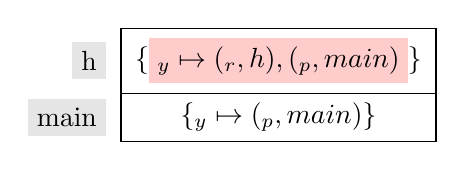
\begin{tikzpicture}[stack/.style={rectangle split, rectangle split parts=#1, draw, anchor=center, text centered},
        scope/.style={fill=gray!20, anchor=center}]
    \node[stack=2, minimum width=4.0cm] (s) {
    \nodepart{one} \{\colorbox{red!20}{$\Blockvar_y \mapsto \onlyread{\set{(\Blockvar_r, \scope{h}), (\Blockvar_p, \scope{main})}}$}\}
    \nodepart{two} \{$\Blockvar_y \mapsto \restricted{\set{(\Blockvar_p, \scope{main})}}$\}
    };
    \node[scope, left=5pt of s.one west]   {\scope{h}};
    \node[scope, left=5pt of s.two west]   {\scope{main}};
    \end{tikzpicture}   
}
\end{minipage}
\end{figure}

\end{frame}

% ---- 


\begin{frame}[fragile]
\frametitle{Aliasing loads (TMU)}
\begin{minted}[escapeinside=||,mathescape=true]{c}
// Scope $\scope{h}$
void h(int* q, int* restrict r, int* restrict s) {
    *q = *r + |\colorbox{red!20}{*s}|; 
}
\end{minted}
\vspace*{-1cm}
\begin{figure}[!h]
\begin{minipage}[t]{.36\textwidth}

\begin{minted}[escapeinside=||,mathescape=true]{c}
// Scope $\scope{main}$
int main() {
    int x, y;
    int* restrict p = &y;
    *p = 0;
    h(&x, p, p);
}
\end{minted}
\end{minipage}%
\begin{minipage}{.64\textwidth}
\colorbox{red!20}{$\onlyread{\set{(\Blockvar_\text{\textcolor{blue}{$r$}}, \scope{h}), (\Blockvar_p, \scope{main})}} \joinsym $} \\
\colorbox{red!20}{$\onlyread{\set{(\Blockvar_\text{\textcolor{blue}{$s$}}, \scope{h}), (\Blockvar_p, \scope{main})}} = ...$}
\\

\executionannotation
{
\{..., \\\  $\Blockvar_r \mapsto \ptr{(\Blockvar_y, \set{(\Blockvar_r, \scope{h}), (\Blockvar_p, \scope{main})})} $, \\
         \ $\Blockvar_s \mapsto \ptr{(\Blockvar_y, \set{(\Blockvar_s, \scope{h}), (\Blockvar_p, \scope{main})})}$ \}
}
{
    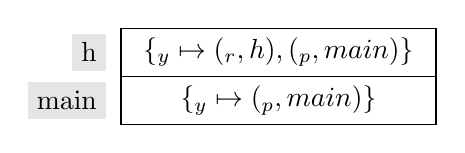
\begin{tikzpicture}[stack/.style={rectangle split, rectangle split parts=#1, draw, anchor=center, text centered},
        scope/.style={fill=gray!20, anchor=center}]
    \node[stack=2, minimum width=4.0cm] (s) {
    \nodepart{one} \{$\Blockvar_y \mapsto \onlyread{\set{(\Blockvar_r, \scope{h}), (\Blockvar_p, \scope{main})}}$\}
    \nodepart{two} \{$\Blockvar_y \mapsto \restricted{\set{(\Blockvar_p, \scope{main})}}$\}
    };
    \node[scope, left=5pt of s.one west]   {\scope{h}};
    \node[scope, left=5pt of s.two west]   {\scope{main}};
    \end{tikzpicture}   
}
\end{minipage}
\end{figure}

\end{frame}


% ----


\begin{frame}[fragile]
\frametitle{Aliasing loads (TMU)}
\centering
\colorbox{red!20}{$\onlyread{\set{(\Blockvar_\text{\textcolor{blue}{$r$}}, \scope{h}), (\Blockvar_p, \scope{main})}} \joinsym \ \onlyread{\set{(\Blockvar_\text{\textcolor{blue}{$s$}}, \scope{h}), (\Blockvar_p, \scope{main})}} = \unrestricted$}

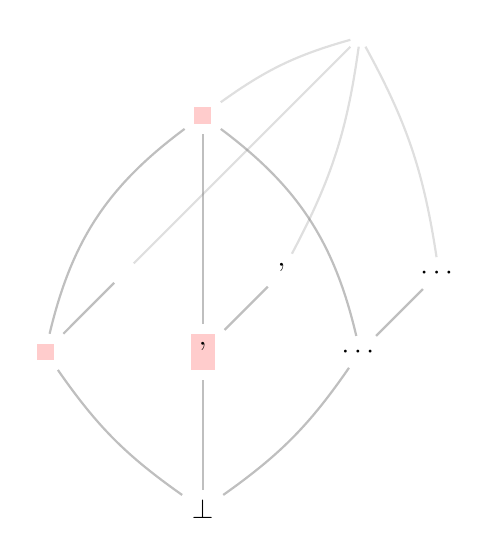
\begin{tikzpicture}
    \node (ub)     at (7,5) {\rsub};
    \node (un)     at (5,4) {\colorbox{red!20}{\unresabbr}};
    \node (rsbs)   at (4,2) {\resabbr{\Basesvar}};
    \node (rsbs')  at (6,2) {\resabbr{\Basesvar'}};
    \node (rsbs'') at (8,2) {$\cdots$};
    \node (orbs)   at (3,1) {\colorbox{red!20}{\orabbr{\Basesvar}}};
    \node (orbs')  at (5,1) {\colorbox{red!20}{\orabbr{\Basesvar'}}};
    \node (orbs'') at (7,1) {$\cdots$};
    \node (bot)    at (5,-1) {$\bot$};

    \path[thick, black, opacity=0.25]
    (bot) edge[bend left=10] node {} (orbs)
    (bot) edge node {} (orbs')
    (bot) edge[bend right=10] node {} (orbs'')
    
    (orbs) edge node {} (rsbs) 
    (orbs') edge node {} (rsbs')
    (orbs'') edge node {} (rsbs'')  
    
    (orbs) edge[bend left=20] node {} (un)
    (orbs') edge node {} (un)
    (orbs'') edge[bend right=20] node {} (un)

    (rsbs) edge[gray] node {} (ub)
    (rsbs') edge[bend right=10, gray] node {} (ub)
    (rsbs'') edge[bend right=10, gray] node {} (ub)

    (un) edge[bend left=10, gray] node {} (ub);
\end{tikzpicture}

\end{frame}

    
% ---- 


\begin{frame}[fragile]
\frametitle{Aliasing loads (TMU)}
\begin{minted}[escapeinside=||,mathescape=true]{c}
// Scope $\scope{h}$
void h(int* q, int* restrict r, int* restrict s) {
    *q = *r + |\colorbox{red!20}{*s}|; 
}
\end{minted}

\vspace*{-1cm}

\begin{figure}[!h]
\begin{minipage}[t]{.36\textwidth}

\begin{minted}[escapeinside=||,mathescape=true]{c}
// Scope $\scope{main}$
int main() {
    int x, y;
    int* restrict p = &y;
    *p = 0;
    h(&x, p, p);
}
\end{minted}
\end{minipage}%
\begin{minipage}{.64\textwidth}

\executionannotation
{
\{..., \\\  $\Blockvar_r \mapsto \ptr{(\Blockvar_y, \set{(\Blockvar_r, \scope{h}), (\Blockvar_p, \scope{main})})} $, \\
            \ $\Blockvar_s \mapsto \ptr{(\Blockvar_y, \set{(\Blockvar_s, \scope{h}), (\Blockvar_p, \scope{main})})}$ \}
}
{
    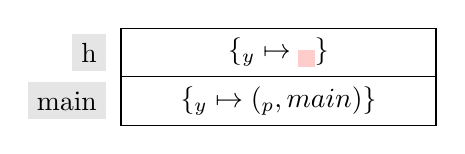
\begin{tikzpicture}[stack/.style={rectangle split, rectangle split parts=#1, draw, anchor=center, text centered},
        scope/.style={fill=gray!20, anchor=center}]
    \node[stack=2, minimum width=4.0cm] (s) {
    \nodepart{one} \{$\Blockvar_y \mapsto \colorbox{red!20}{\unrestricted}$\}
    \nodepart{two} \{$\Blockvar_y \mapsto \restricted{\set{(\Blockvar_p, \scope{main})}}$\}
    };
    \node[scope, left=5pt of s.one west]   {\scope{h}};
    \node[scope, left=5pt of s.two west]   {\scope{main}};
    \end{tikzpicture}   
}
\end{minipage}
\end{figure}

\end{frame}


% ---- 


\begin{frame}[fragile]
\frametitle{Aliasing loads (TMU)}
\begin{minted}[escapeinside=||,mathescape=true]{c}
// Scope $\scope{h}$
void h(int* q, int* restrict r, int* restrict s) {
    *q = *r + *s; 
|\colorbox{red!20}{\}}|
\end{minted}

\vspace*{-1cm}

\begin{figure}[!h]
\begin{minipage}[t]{.36\textwidth}

\begin{minted}[escapeinside=||,mathescape=true]{c}
// Scope $\scope{main}$
int main() {
    int x, y;
    int* restrict p = &y;
    *p = 0;
    h(&x, p, p);
}
\end{minted}
\end{minipage}%
\begin{minipage}{.64\textwidth}

\executionannotation
{
\{..., \\\  $\Blockvar_r \mapsto \ptr{(\Blockvar_y, \set{(\Blockvar_r, \scope{h}), (\Blockvar_p, \scope{main})})} $, \\
            \ $\Blockvar_s \mapsto \ptr{(\Blockvar_y, \set{(\Blockvar_s, \scope{h}), (\Blockvar_p, \scope{main})})}$ \}
}
{
    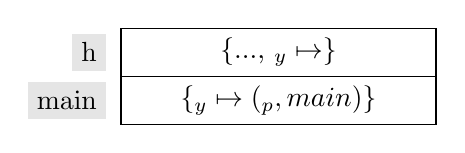
\begin{tikzpicture}[stack/.style={rectangle split, rectangle split parts=#1, draw, anchor=center, text centered},
        scope/.style={fill=gray!20, anchor=center}]
    \node[stack=2, minimum width=4.0cm] (s) {
    \nodepart{one} \{..., $\Blockvar_y \mapsto \unrestricted$\}
    \nodepart{two} \{$\Blockvar_y \mapsto \restricted{\set{(\Blockvar_p, \scope{main})}}$\}
    };
    \node[scope, left=5pt of s.one west]   {\scope{h}};
    \node[scope, left=5pt of s.two west]   {\scope{main}};
    \end{tikzpicture}   
}
\end{minipage}
\end{figure}

\end{frame}

    
% ---- 


\begin{frame}[fragile]
\frametitle{Aliasing loads (TMU)}

\begin{itemize}
    \item \scope{h} is part of the execution of scope \scope{main}
    \item Join the restrict states when \scope{h} terminates!
\end{itemize}
\leavevmode\\
\begin{tikzpicture}[stack/.style={rectangle split, rectangle split parts=#1, draw, anchor=center, text centered},
    scope/.style={fill=gray!20, anchor=center}]
\node[stack=2, minimum width=4.0cm] (s) {
\nodepart{one} \{$\Blockvar_y \mapsto \unrestricted$\}
\nodepart{two} \{$\Blockvar_y \mapsto \restricted{\set{(\Blockvar_p, \scope{main})}}$\}
};
\node[scope, left=5pt of s.one west]   {\scope{h}};
\node[scope, left=5pt of s.two west]   {\scope{main}};

\draw[->, dashed, thick] (s.one east) to[bend left=90, looseness=3] node[right] {$\joinsym$} (s.two east);

\end{tikzpicture}

\end{frame}


\begin{frame}[fragile]
\frametitle{Aliasing loads (TMU)}
\centering
\colorbox{red!20}{$\restricted{\set{(\Blockvar_p, \scope{main})}} \joinsym \unrestricted = \rsub$}

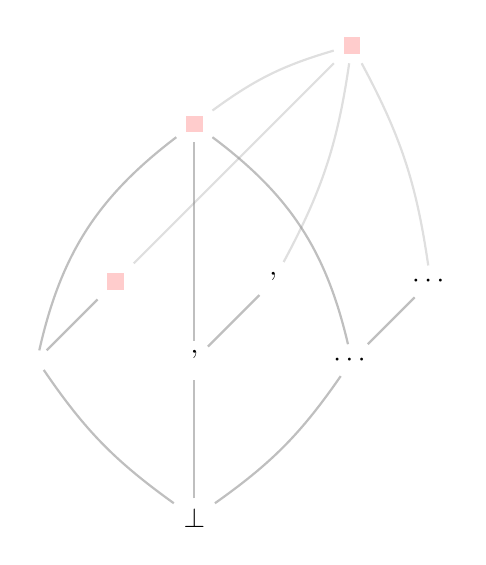
\begin{tikzpicture}
    \node (ub)     at (7,5) {\colorbox{red!20}{\rsub}};
    \node (un)     at (5,4) {\colorbox{red!20}{\unresabbr}};
    \node (rsbs)   at (4,2) {\colorbox{red!20}{\resabbr{\Basesvar}}};
    \node (rsbs')  at (6,2) {\resabbr{\Basesvar'}};
    \node (rsbs'') at (8,2) {$\cdots$};
    \node (orbs)   at (3,1) {\orabbr{\Basesvar}};
    \node (orbs')  at (5,1) {\orabbr{\Basesvar'}};
    \node (orbs'') at (7,1) {$\cdots$};
    \node (bot)    at (5,-1) {$\bot$};

    \path[thick, black, opacity=0.25]
    (bot) edge[bend left=10] node {} (orbs)
    (bot) edge node {} (orbs')
    (bot) edge[bend right=10] node {} (orbs'')
    
    (orbs) edge node {} (rsbs) 
    (orbs') edge node {} (rsbs')
    (orbs'') edge node {} (rsbs'')  
    
    (orbs) edge[bend left=20] node {} (un)
    (orbs') edge node {} (un)
    (orbs'') edge[bend right=20] node {} (un)

    (rsbs) edge[gray] node {} (ub)
    (rsbs') edge[bend right=10, gray] node {} (ub)
    (rsbs'') edge[bend right=10, gray] node {} (ub)

    (un) edge[bend left=10, gray] node {} (ub);
\end{tikzpicture}

\end{frame}


% ----


\begin{frame}[fragile]
\frametitle{Aliasing loads (TMU)}
\begin{itemize}
    \item The fundamental problem with $\unrestricted$ is \textbf{information loss}
    \item Idea: \textbf{remove} $\unrestricted$ entirely and promote $(\onlyread{\Basesvar})$ to $(\onlyread{\textdom{fbas}})$ with $\textdom{fbas} \in \Set{\Bases}$, \ie
    a \textbf{family of sets of bases}
    \begin{itemize}
        \item Every set of the family represents a pointer used for a load \\
        \item if $|\Basesfamvar| > 1$              \qquad the semantics of $\unrestricted$ apply
        \item if $\Basesfamvar = \set{\Basesvar}$ \;   the semantics of $(\onlyread{\Basesvar})$ apply
    \end{itemize}
\end{itemize}
\end{frame}

% ---- 


\begin{frame}[fragile]
\frametitle{Aliasing loads (TMU)}
\begin{minted}[escapeinside=||,mathescape=true]{c}
// Scope $\scope{h}$
void h(int* q, int* restrict r, int* restrict s) {
    *q = *r + |\colorbox{red!20}{*s}|; 
}
\end{minted}
\vspace*{-1cm}
\begin{figure}[!h]
\begin{minipage}[t]{.36\textwidth}

\begin{minted}[escapeinside=||,mathescape=true]{c}
// Scope $\scope{main}$
int main() {
    int x, y;
    int* restrict p = &y;
    *p = 0;
    h(&x, p, p);
}
\end{minted}
\end{minipage}%
\begin{minipage}{.64\textwidth}
\colorbox{red!20}{$\onlyread{\set{\set{(\Blockvar_\text{\textcolor{blue}{$r$}}, \scope{h}), (\Blockvar_p, \scope{main})}}} \joinsym $} \\
\colorbox{red!20}{$\onlyread{\set{\set{(\Blockvar_\text{\textcolor{blue}{$s$}}, \scope{h}), (\Blockvar_p, \scope{main})}}} = ...$}
\\

\executionannotation
{
\{..., \\\  $\Blockvar_r \mapsto \ptr{(\Blockvar_y, \set{(\Blockvar_r, \scope{h}), (\Blockvar_p, \scope{main})})} $, \\
            \ $\Blockvar_s \mapsto \ptr{(\Blockvar_y, \set{(\Blockvar_s, \scope{h}), (\Blockvar_p, \scope{main})})}$ \}
}
{
    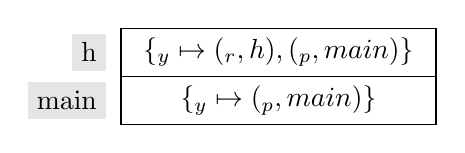
\begin{tikzpicture}[stack/.style={rectangle split, rectangle split parts=#1, draw, anchor=center, text centered},
        scope/.style={fill=gray!20, anchor=center}]
    \node[stack=2, minimum width=4.0cm] (s) {
    \nodepart{one} \{$\Blockvar_y \mapsto \onlyread{\set{\set{(\Blockvar_r, \scope{h}), (\Blockvar_p, \scope{main})}}}$\}
    \nodepart{two} \{$\Blockvar_y \mapsto \restricted{\set{(\Blockvar_p, \scope{main})}}$\}
    };
    \node[scope, left=5pt of s.one west]   {\scope{h}};
    \node[scope, left=5pt of s.two west]   {\scope{main}};
    \end{tikzpicture}   
}
\end{minipage}
\end{figure}

\end{frame}


% ---- 


\begin{frame}[fragile]
\frametitle{Aliasing loads (TMU)}
\centering
\colorbox{red!20}{$\onlyread{\set{\set{(\Blockvar_\text{\textcolor{blue}{$r$}}, \scope{h}), (\Blockvar_p, \scope{main})}}} \joinsym \onlyread{\set{\set{(\Blockvar_\text{\textcolor{blue}{$s$}}, \scope{h}), (\Blockvar_p, \scope{main})}}} = ...$}
\\

\begin{minipage}{.43\textwidth}
\begin{itemize}
    \item The updated symmetric \joinsym \ operation (simplified)
    \item $\Basesvar \neq \Basesvar'$
\end{itemize}
\end{minipage}%
\begin{minipage}{.57\textwidth}
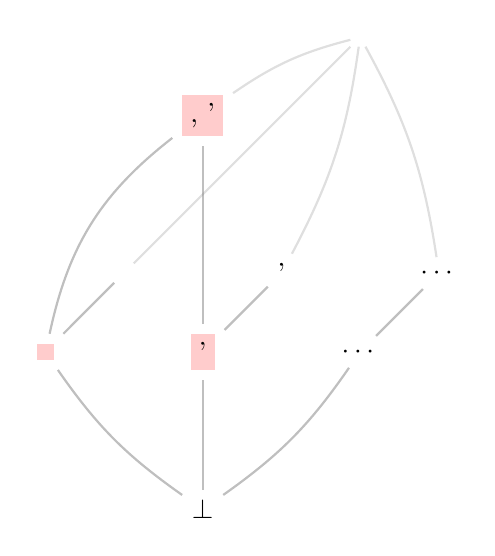
\begin{tikzpicture}
    \node (ub)     at (7,5) {\rsub};
    \node (un)     at (5,4) {\colorbox{red!20}{\orabbr{\set{\Basesvar, \Basesvar'}}}};
    \node (rsbs)   at (4,2) {\resabbr{\Basesvar}};
    \node (rsbs')  at (6,2) {\resabbr{\Basesvar'}};
    \node (rsbs'') at (8,2) {$\cdots$};
    \node (orbs)   at (3,1) {\colorbox{red!20}{\orabbr{\set{\Basesvar}}}};
    \node (orbs')  at (5,1) {\colorbox{red!20}{\orabbr{\set{\Basesvar'}}}};
    \node (orbs'') at (7,1) {$\cdots$};
    \node (bot)    at (5,-1) {$\bot$};

    \path[thick, black, opacity=0.25]
    (bot) edge[bend left=10] node {} (orbs)
    (bot) edge node {} (orbs')
    (bot) edge[bend right=10] node {} (orbs'')
    
    (orbs) edge node {} (rsbs) 
    (orbs') edge node {} (rsbs')
    (orbs'') edge node {} (rsbs'')  
    
    (orbs) edge[bend left=20] node {} (un)
    (orbs') edge node {} (un)
    % (orbs'') edge[bend right=20] node {} (un)

    (rsbs) edge[gray] node {} (ub)
    (rsbs') edge[bend right=10, gray] node {} (ub)
    (rsbs'') edge[bend right=10, gray] node {} (ub)

    (un) edge[bend left=10, gray] node {} (ub);
\end{tikzpicture}
\end{minipage}

\end{frame}




% ---- 


\begin{frame}[fragile]
\frametitle{Aliasing loads (TMU)}
\begin{minted}[escapeinside=||,mathescape=true]{c}
// Scope $\scope{h}$
void h(int* q, int* restrict r, int* restrict s) {
    *q = *r + |\colorbox{red!20}{*s}|; 
}
\end{minted}
\vspace*{-1cm}
\begin{figure}[!h]
\begin{minipage}[t]{.36\textwidth}

\begin{minted}[escapeinside=||,mathescape=true]{c}
// Scope $\scope{main}$
int main() {
    int x, y;
    int* restrict p = &y;
    *p = 0;
    h(&x, p, p);
}
\end{minted}
\end{minipage}%
\begin{minipage}{.64\textwidth}

\executionannotation
{
\{..., \\\  $\Blockvar_r \mapsto \ptr{(\Blockvar_y, \set{(\Blockvar_r, \scope{h}), (\Blockvar_p, \scope{main})})} $, \\
            \ $\Blockvar_s \mapsto \ptr{(\Blockvar_y, \set{(\Blockvar_s, \scope{h}), (\Blockvar_p, \scope{main})})}$ \}
}
{
    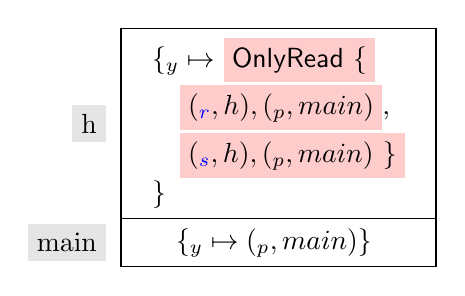
\begin{tikzpicture}[stack/.style={rectangle split, rectangle split parts=#1, draw, anchor=center, text centered,align=left},
        scope/.style={fill=gray!20, anchor=center}]
    \node[stack=2, minimum width=4.0cm] (s) {
    \nodepart[align=left]{one} \{$\Blockvar_y \mapsto$ \colorbox{red!20}{$\mathsf{OnlyRead}$ \{} \\
                                \quad \colorbox{red!20}{$\set{(\Blockvar_\text{\textcolor{blue}{$r$}}, \scope{h}), (\Blockvar_p, \scope{main})}$}, \\
                                \quad \colorbox{red!20}{$\set{(\Blockvar_\text{\textcolor{blue}{$s$}}, \scope{h}), (\Blockvar_p, \scope{main})}$ \}} \\ \}
                    
                   
    \nodepart{two} \{$\Blockvar_y \mapsto \restricted{\set{(\Blockvar_p, \scope{main})}}$\}
    };
    \node[scope, left=5pt of s.one west]   {\scope{h}};
    \node[scope, left=5pt of s.two west]   {\scope{main}};
    \end{tikzpicture}   
}
\end{minipage}
\end{figure}

\end{frame}


% ---- 


\begin{frame}[fragile]
\frametitle{Aliasing loads (TMU)}
\begin{minted}[escapeinside=||,mathescape=true]{c}
// Scope $\scope{h}$
void h(int* q, int* restrict r, int* restrict s) {
    *q = *r + *s; 
|\colorbox{red!20}{\}}|
\end{minted}
\vspace*{-1cm}
\begin{figure}[!h]
\begin{minipage}[t]{.36\textwidth}

\begin{minted}[escapeinside=||,mathescape=true]{c}
// Scope $\scope{main}$
int main() {
    int x, y;
    int* restrict p = &y;
    *p = 0;
    h(&x, p, p);
}
\end{minted}
\end{minipage}%
\begin{minipage}{.64\textwidth}

\executionannotation
{
\{..., \\\  $\Blockvar_r \mapsto \ptr{(\Blockvar_y, \set{(\Blockvar_r, \scope{h}), (\Blockvar_p, \scope{main})})} $, \\
            \ $\Blockvar_s \mapsto \ptr{(\Blockvar_y, \set{(\Blockvar_s, \scope{h}), (\Blockvar_p, \scope{main})})}$ \}
}
{
    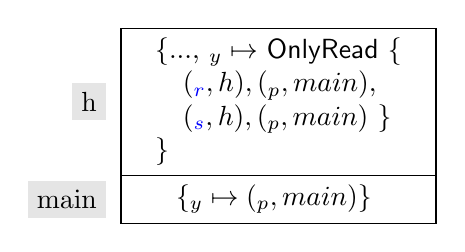
\begin{tikzpicture}[stack/.style={rectangle split, rectangle split parts=#1, draw, anchor=center, text centered,align=left},
        scope/.style={fill=gray!20, anchor=center}]
    \node[stack=2, minimum width=4.0cm] (s) {
    \nodepart[align=left]{one} \{...,  $\Blockvar_y \mapsto$ $\mathsf{OnlyRead}$ \{ \\
                                \quad $\set{(\Blockvar_\text{\textcolor{blue}{$r$}}, \scope{h}), (\Blockvar_p, \scope{main})}$, \\
                                \quad $\set{(\Blockvar_\text{\textcolor{blue}{$s$}}, \scope{h}), (\Blockvar_p, \scope{main})}$ \} \\ \}
                    
                    
    \nodepart{two} \{$\Blockvar_y \mapsto \restricted{\set{(\Blockvar_p, \scope{main})}}$\}
    };
    \node[scope, left=5pt of s.one west]   {\scope{h}};
    \node[scope, left=5pt of s.two west]   {\scope{main}};
    \end{tikzpicture}   
}
\end{minipage}
\end{figure}

\end{frame}



% ---- 


\begin{frame}[fragile,label=current]
\frametitle{Aliasing loads (TMU)}
\centering

\begin{itemize}
    \item Recall that the restrict rules only apply during the \textbf{scope a restrict pointer is alive}
    \item Filtering: when joining between scopes, remove bases from the expired scope \scope{h}
\end{itemize}

\pause

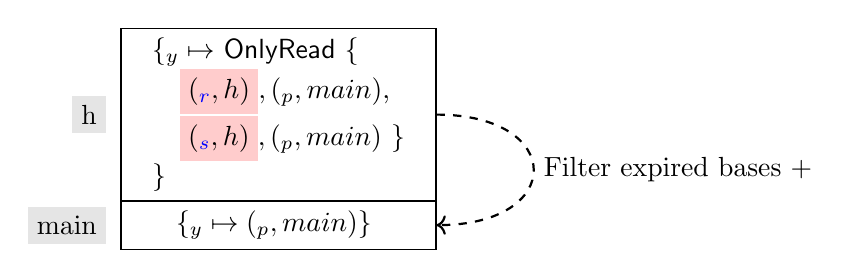
\begin{tikzpicture}[stack/.style={rectangle split, rectangle split parts=#1, draw, anchor=center, text centered,align=left},
    scope/.style={fill=gray!20, anchor=center}]
\node[stack=2, minimum width=4.0cm] (s) {
\nodepart[align=left]{one} \{$\Blockvar_y \mapsto$ $\mathsf{OnlyRead}$ \{ \\
                            \quad $\set{\text{\colorbox{red!20}{$(\Blockvar_\text{\textcolor{blue}{$r$}}, \scope{h})$}}, (\Blockvar_p, \scope{main})}$, \\
                            \quad $\set{\text{\colorbox{red!20}{$(\Blockvar_\text{\textcolor{blue}{$s$}}, \scope{h})$}}, (\Blockvar_p, \scope{main})}$ \} \\ \}
                
               
\nodepart{two} \{$\Blockvar_y \mapsto \restricted{\set{(\Blockvar_p, \scope{main})}}$\}
};
\node[scope, left=5pt of s.one west]   {\scope{h}};
\node[scope, left=5pt of s.two west]   {\scope{main}};

\draw[->, dashed, thick] (s.one east) to[bend left=90, looseness=3] node[right] {Filter expired bases + $\joinsym$} (s.two east);


\end{tikzpicture}

\leavevmode \\

\begin{itemize}
    \item Filtered state: $\onlyread{\set{\set{(\Blockvar_p, \scope{main})}}}$
    \item $\onlyread{\set{\set{(\Blockvar_p, \scope{main})}}} \joinsym \restricted{\set{(\Blockvar_p, \scope{main})}} = ...$
\end{itemize}

\end{frame}

% ---- 


\begin{frame}[fragile]
\frametitle{Aliasing loads (TMU)}
\centering
\colorbox{red!20}{$\onlyread{\set{\set{(\Blockvar_p, \scope{main})}}} \joinsym \restricted{\set{(\Blockvar_p, \scope{main})}} = \restricted{\set{(\Blockvar_p, \scope{main})}}$}
\\

\begin{minipage}{.43\textwidth}
\begin{itemize}
    \item The updated symmetric \joinsym \ operation (simplified)
    \item $\Basesvar \neq \Basesvar'$
\end{itemize}
\end{minipage}%
\begin{minipage}{.57\textwidth}
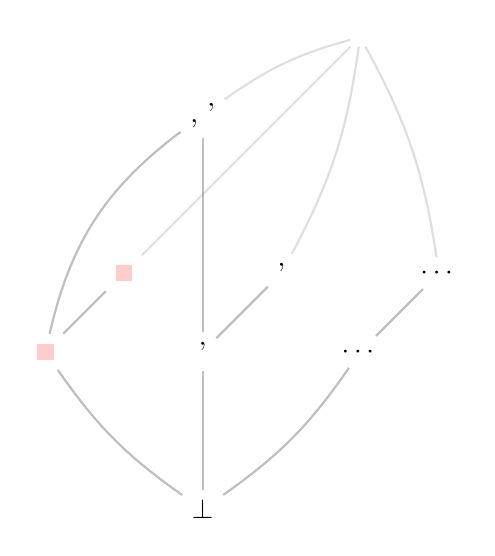
\begin{tikzpicture}
    \node (ub)     at (7,5) {\rsub};
    \node (un)     at (5,4) {\orabbr{\set{\Basesvar, \Basesvar'}}};
    \node (rsbs)   at (4,2) {\colorbox{red!20}{\resabbr{\Basesvar}}};
    \node (rsbs')  at (6,2) {\resabbr{\Basesvar'}};
    \node (rsbs'') at (8,2) {$\cdots$};
    \node (orbs)   at (3,1) {\colorbox{red!20}{\orabbr{\set{\Basesvar}}}};
    \node (orbs')  at (5,1) {\orabbr{\set{\Basesvar'}}};
    \node (orbs'') at (7,1) {$\cdots$};
    \node (bot)    at (5,-1) {$\bot$};

    \path[thick, black, opacity=0.25]
    (bot) edge[bend left=10] node {} (orbs)
    (bot) edge node {} (orbs')
    (bot) edge[bend right=10] node {} (orbs'')
    
    (orbs) edge node {} (rsbs) 
    (orbs') edge node {} (rsbs')
    (orbs'') edge node {} (rsbs'')  
    
    (orbs) edge[bend left=20] node {} (un)
    (orbs') edge node {} (un)
    % (orbs'') edge[bend right=20] node {} (un)

    (rsbs) edge[gray] node {} (ub)
    (rsbs') edge[bend right=10, gray] node {} (ub)
    (rsbs'') edge[bend right=10, gray] node {} (ub)

    (un) edge[bend left=10, gray] node {} (ub);
\end{tikzpicture}
\end{minipage}

\end{frame}


% ---- 


\begin{frame}[fragile]
\frametitle{Aliasing loads (TMU)}
\begin{itemize}
    \item Loads via aliased pointers are now permitted \smiley{}
    \item Achieved our goal of relaxing the semantics for this problem to give \textbf{less UB}, \textbf{consistent} with the ISO standard
\end{itemize}
\end{frame}


\begin{frame}
\frametitle{Crestrict refinements}
\begin{itemize}
\item Too much undefined behavior (TMU)
    \begin{itemize}
        \item[$\greentriangleright$] Aliasing loads: \textbf{adjust restrict states and $\joinsym$ lattice}
        \item Returning restrict pointers: \textbf{track active scopes and filter pointer values}
    \end{itemize}
\item Too little undefined behavior (TLU)
    \begin{itemize}
        \item Array of restrict pointers: \textbf{refine bases granularity to offsets}
        \item Nested restrict pointers: \textbf{missing subclause and pointer values as a tree structure}
        \item Semantic preservation under inlining: \textbf{deferred $\rightarrow$ eager check}
        \item Call to free: \textbf{update the restrict state}
    \end{itemize}
\end{itemize}

\begin{itemize}
    \item \textbf{Consistency}, goal 2 \cmark (\ie, to the best of our knowledge)
\end{itemize}

\end{frame}



\begin{frame}
\frametitle{Evaluation}
\begin{itemize}
    \item Implemented the semantics in an interpreter, written in Rust (\textbf{executable}, goal 3 \cmark)
    \item A (public) test suite dedicated to restrict does not exist
    \item Created our own suite of 96 tests, build around common restrict use cases and the discussed problems
\end{itemize}
\end{frame}



\begin{frame}
\frametitle{Conclusion}
\begin{itemize}
    \item Redeveloped the restrict fragment of the \cink semantics in a functional style (4)
    \item We argued it has six consistency problems
    \item We proposed changes to the semantic domains and rules to solve them (2)
    \item The new Crestrict semantics (1,3) were implemented in an interpreter and evaluated under a more extensive test suite   
\end{itemize}

\begin{enumerate}
    \item \textcolor{ao}{Unambiguous: \cmark}
    \item \textcolor{ao}{Consistent: \cmark}
    \item \textcolor{ao}{Executable: \cmark}
    \item \textcolor{ao}{Suitable: \cmark}
\end{enumerate}

\end{frame}


\begin{frame}
\frametitle{Future work}
\begin{itemize}
    \item Assignments between restrict pointers
    \item A more complete language
    \item Proving optimizations correct (the sequal of goal 4)
    \item ...
\end{itemize}
\end{frame}



% EXTRA SLIDES


\begin{frame}
\frametitle{}
\end{frame}


\begin{frame}[fragile]
\frametitle{Returning restrict pointers (TMU)}

\begin{minted}[escapeinside=||,mathescape=true]{c}
int* as_mut_ptr(int* restrict v) {
    return v;
}
\end{minted}

\vspace*{-1cm}

\begin{figure}[!h]
\begin{minipage}[t]{.4\textwidth}

\begin{minted}[escapeinside=||,mathescape=true]{c}
int main() {
    int a;

    int* p = as_mut_ptr(&a);
    int* q = as_mut_ptr(&a);

    *p = 0;
    |\colorbox{red!20}{*q = 0;}|
}

\end{minted}
\end{minipage}%
\begin{minipage}{.6\textwidth}
\colorbox{red!20}{$\restricted{\set{(\Blockvar_{v2}, \scope{as\_mut\_ptr\_2})}} \joinsym$} \\
\colorbox{red!20}{$\restricted{\set{(\Blockvar_{v1}, \scope{as\_mut\_ptr\_1})}} = \rsub$} \\

\executionannotation
{
    \{$\Blockvar_a \mapsto 0$, \\
        \ $\Blockvar_p \mapsto \ptr{(\Blockvar_a, \set{(\Blockvar_{v1}, \scope{as\_mut\_ptr\_1})})}$, \\
        \ $\Blockvar_q \mapsto \ptr{(\Blockvar_a, \set{(\Blockvar_{v2}, \scope{as\_mut\_ptr\_2})})}$
    \}
    }
{
    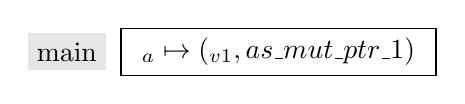
\begin{tikzpicture}[stack/.style={rectangle split, rectangle split parts=#1, draw, anchor=center, text centered},
        scope/.style={fill=gray!20, anchor=center}]
    \node[stack=1, minimum width=4.0cm] (s) {
        \nodepart{one} $\set{\Blockvar_a \mapsto \restricted{\set{(\Blockvar_{v1}, \scope{as\_mut\_ptr\_1})}}}$
    };

    \node[scope, left=5pt of s.one west]   {\scope{main}};
    

    \end{tikzpicture}
}
\end{minipage}
\end{figure}

\end{frame}



\begin{frame}[fragile]
\frametitle{Array of restrict pointers (TLU)}
\begin{minipage}{.45\textwidth}
\begin{minted}[escapeinside=||,mathescape=true]{c}
// Scope $\scope{main}$
int main() {
    int x;
    int* restrict a[2] = {&x, &x};

    *(a[0]) = 10;
    |\colorbox{red!20}{*(a[1]) = 11;}|
}
\end{minted}
\end{minipage}%
\begin{minipage}{.55\textwidth}
\colorbox{red!20}{$\restricted{\set{(\Blockvar_a, \scope{main})}} \joinsym \restricted{\set{(\Blockvar_a, \scope{main})}}$} \\
\colorbox{red!20}{$= \restricted{\set{(\Blockvar_a, \scope{main})}}$} \\

\executionannotation
{
    \{$\Blockvar_x \mapsto 10$, \\
      \ $\Blockvar_a \mapsto \{\ptr{(\Blockvar_x, \set{(\Blockvar_a, \scope{main})})}$,\\ 
      \ \qquad\quad $\ptr{(\Blockvar_x, \set{(\Blockvar_a, \scope{main})})}$ \}\}  
}
{
    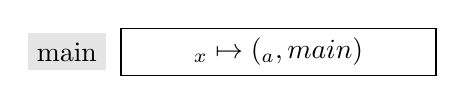
\begin{tikzpicture}[stack/.style={rectangle split, rectangle split parts=#1, draw, anchor=center, text centered},
        scope/.style={fill=gray!20, anchor=center}]
    \node[stack=1, minimum width=4.0cm] (s) {
        \nodepart{one} $\set{\Blockvar_x \mapsto \restricted{\set{(\Blockvar_a, \scope{main})}}}$
    };

    \node[scope, left=5pt of s.one west]   {\scope{main}};
    \end{tikzpicture}
}
\end{minipage}
\end{frame}


\begin{frame}[fragile]
\frametitle{Semantic preservation under inlining (TLU)}
\begin{minted}[escapeinside=||,mathescape=true]{c}
// Scope $\scope{foo}$
void foo(int* q) {
    *q = 0;
    |\colorbox{red!20}{while(1) \{\}}|
    // Never terminates
}
\end{minted}


\begin{minipage}{.4\textwidth}
\begin{minted}[escapeinside=||,mathescape=true]{c}
// Scope $\scope{main}$
int main() {
    int x = 5;
    int* restrict p = &x;
    *p;
    foo(&x);
}
\end{minted}
\end{minipage}%
\begin{minipage}{.6\textwidth}
\executionannotation
{
    \{$\Blockvar_x \mapsto 5$, \\
     \ $\Blockvar_p \mapsto \ptr{(\Blockvar_x, \set{(\Blockvar_p, \scope{main})})}$, \\
     \ $\Blockvar_q \mapsto \ptr{(\Blockvar_x, \emptyset)}$
    \}
}
{
    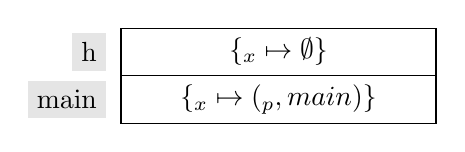
\begin{tikzpicture}[stack/.style={rectangle split, rectangle split parts=#1, draw, anchor=center, text centered},
        scope/.style={fill=gray!20, anchor=center}]
    \node[stack=2, minimum width=4.0cm] (s) {
    \nodepart{one} \{$\Blockvar_x \mapsto \restricted{\emptyset}$\}
    \nodepart{two} \{$\Blockvar_x \mapsto \onlyread{\set{(\Blockvar_p, \scope{main})}}$\}
    };
    \node[scope, left=5pt of s.one west]   {\scope{h}};
    \node[scope, left=5pt of s.two west]   {\scope{main}};
    \end{tikzpicture}
}
\end{minipage}

\end{frame}


\begin{frame}[fragile]
\frametitle{Semantic preservation under inlining (TLU)}
\begin{minipage}{.4\textwidth}
\begin{minted}[escapeinside=||,mathescape=true]{c}
// foo is inlined into main
// Scope $\scope{main}$
int main() {
    int x = 5;
    int* restrict p = &x;
    *p;
    int* q = &x;
    |\colorbox{red!20}{*q = 0;}|
    while (1) {}
}
\end{minted}
\end{minipage}%
\begin{minipage}{.6\textwidth}
\colorbox{red!20}{$\restricted{\emptyset} \joinsym \onlyread{\set{(\Blockvar_p, \scope{main})}} = \rsub$} \\

\executionannotation
{
    \{$\Blockvar_x \mapsto 5$, \\
     \ $\Blockvar_p \mapsto \ptr{(\Blockvar_x, \set{(\Blockvar_p, \scope{main})})}$, \\
     \ $\Blockvar_q \mapsto \ptr{(\Blockvar_x, \emptyset)}$
    \}
}
{
    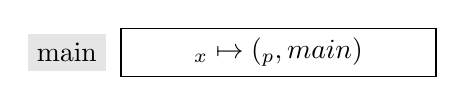
\begin{tikzpicture}[stack/.style={rectangle split, rectangle split parts=#1, draw, anchor=center, text centered},
        scope/.style={fill=gray!20, anchor=center}]
    \node[stack=1, minimum width=4.0cm] (s) {
        \nodepart{one} $\set{\Blockvar_x \mapsto \onlyread{\set{(\Blockvar_p, \scope{main})}}}$
    };

    \node[scope, left=5pt of s.one west]   {\scope{main}};
    \end{tikzpicture}
}
\end{minipage}

\end{frame}


\begin{frame}[fragile]
\frametitle{Call to free (TLU)}
\begin{minipage}{.5\textwidth}
\begin{minted}[escapeinside=||,mathescape=true]{c}
// Scope $\scope{bar}$
void bar(int* s) {
    free(s);
}
// Scope $\scope{foo}$
void foo(int* restrict q, int* r) {
    |\colorbox{red!20}{*q = 5;}|
    bar(r);
}
// Scope $\scope{main}$
int main() {
    // Stored at $\Blockvar_v$
    int* p = malloc(sizeof(int));
    foo(p, p);
}
\end{minted}
\end{minipage}%
\begin{minipage}{.5\textwidth}
\executionannotation
{
\{$\Blockvar_v \mapsto 5$, \\
   \ $\Blockvar_p \mapsto \ptr{(\Blockvar_v, \emptyset)}$, \\
    \ $\Blockvar_q \mapsto \ptr{(\Blockvar_v, \set{(\Blockvar_q, \scope{foo})})}$, \\
    \ $\Blockvar_r \mapsto \ptr{(\Blockvar_v, \emptyset)}$ \}
}
{
    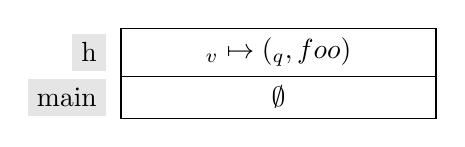
\begin{tikzpicture}[stack/.style={rectangle split, rectangle split parts=#1, draw, anchor=center, text centered},
        scope/.style={fill=gray!20, anchor=center}]
    \node[stack=2, minimum width=4.0cm] (s) {
    \nodepart{one} $\set{\Blockvar_v \mapsto \restricted{(\Blockvar_q, \scope{foo})}}$
    \nodepart{two} $\emptyset$
    };
    \node[scope, left=5pt of s.one west]   {\scope{h}};
    \node[scope, left=5pt of s.two west]   {\scope{main}};
    \end{tikzpicture}   
}
\end{minipage}

\end{frame}



\begin{frame}[fragile]
\frametitle{Nested restrict pointers (TLU)}
\begin{minipage}{0.7\textwidth}
\begin{minted}[escapeinside=||,mathescape=true,linenos]{c}
// Scope $\scope{foo}$
int foo(int *restrict *restrict p, int *restrict *restrict q) {
    **p = 10;
    **q = 11;
    return **p; // Optimized to 10 by GCC
}
// Scope $\scope{main}$
int main() {
    int x;
    int* xp = &x;
    foo(&xp, &xp);
}
\end{minted}
\end{minipage}%
\begin{minipage}[t]{0.3\textwidth}
\begin{tikzpicture}
    \node (pq) {\mintinline{c}{p,q}};
    \node[right of = pq] (xp) {\mintinline{c}{xp}};
    \node[right of = xp] (x) {\mintinline{c}{x}};

    \draw[->] (pq) -- (xp);
    \draw[->] (xp) -- (x);
\end{tikzpicture}
\end{minipage}

\begin{itemize}
    \item UB due to a subtle subclause of the standard
\end{itemize}

\end{frame}


% Restrict definition
\begin{frame}
\frametitle{Restrict definition (simplified)}
\begin{itemize}
    % \item A type qualifier for \textbf{pointer types}, \eg \mintinline{c}{int* restrict p;}
    \item A pointer is ``based on'' a restrict pointer if it depends on its value: \\
        \mintinline[mathescape=true]{c}{int x; int* restrict p = &x; int* q = p; // $q$ is based on $p$}  
    \item A \textbf{promise} from the programmer to the compiler that a restrict qualified pointer and pointers ``based on" it will \textbf{not alias} with other pointers during the \textbf{scope} it is alive if:
            \begin{itemize}
                \item The pointer is used to \textbf{access} the object it points to
                \item The object pointed to is \textbf{modified} (by any means)
            \end{itemize}
    \item \colorbox{red!20}{``Modifications of the object pointed to by a restrict pointer are considered to modify} \\ \colorbox{red!20}{the restrict pointer object itself"}
\end{itemize}
\end{frame}




\begin{frame}[fragile]
\frametitle{Nested restrict pointers (TLU)}
\begin{itemize}
    \item What does ``modifications of the object pointed to by a restrict pointer are considered to modify the restrict pointer object itself" mean?
    \item Modifications are represented by the restrict state $\restrictedn$
\end{itemize}

\pause

\begin{figure}[h]
\centering
\begin{minipage}{.5\textwidth}
\begin{minted}[escapeinside=||,mathescape=true]{c}
// Scope $\scope{main}$
{
int x; // $\&x = \Blockvar_x$
int* restrict p = &x; // $\&p = \Blockvar_p$
|\colorbox{red!20}{*p = 10;}| // Modification
}
\end{minted}
\end{minipage}%
\begin{minipage}{.5\textwidth}
\executionannotation
{
    \{$\Blockvar_x \mapsto \colorbox{red!20}{10}$, \\
      \ $\Blockvar_p \mapsto \ptr{(\Blockvar_x, \set{(\Blockvar_p, \scope{main})})}$
    \}
}
{
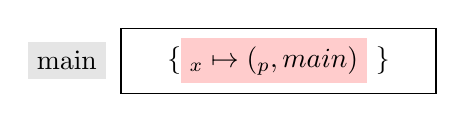
\begin{tikzpicture}[stack/.style={rectangle split, rectangle split parts=#1, draw, anchor=center, text centered},
    scope/.style={fill=gray!20, anchor=center}]

\node[stack=1, minimum width=4.0cm] (s) {
    \nodepart{one} \{\colorbox{red!20}{$\Blockvar_x \mapsto \restricted{\set{(\Blockvar_p, \scope{main})}}$} \}

};

\node[scope, left=5pt of s.one west]   {\scope{main}};

\end{tikzpicture}
}
\end{minipage}
\end{figure}


\end{frame}

\begin{frame}[fragile]
\frametitle{Nested restrict pointers (TLU)}
\begin{itemize}
    \item What does ``modifications of the object pointed to by a restrict pointer are considered to modify the restrict pointer object itself" mean?
    \item Modifications are represented by the restrict state \colorbox{blue!20}{$\restrictedn$}
\end{itemize}

\begin{figure}[h]
\centering
\begin{minipage}{.5\textwidth}
\begin{minted}[escapeinside=||,mathescape=true]{c}
// Scope $\scope{main}$
{
int x; // $\&x = \Blockvar_x$
int* restrict p = &x; // $\&p = \Blockvar_p$
|\colorbox{red!20}{*p = 10;}| // Modification
}
\end{minted}
\end{minipage}%
\begin{minipage}{.5\textwidth}
\executionannotation
{
    \{$\Blockvar_x \mapsto \colorbox{red!20}{10}$, \\
        \ $\Blockvar_p \mapsto \ptr{(\Blockvar_x, \set{(\Blockvar_p, \scope{main})})}$
    \}
}
{
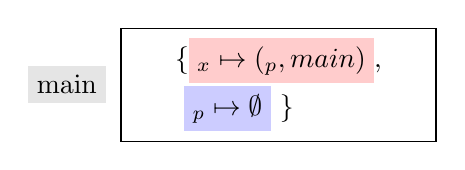
\begin{tikzpicture}[stack/.style={rectangle split, rectangle split parts=#1, draw, anchor=center, text centered},
    scope/.style={fill=gray!20, anchor=center}]

\node[stack=1, minimum width=4.0cm] (s) {
    \nodepart[align=left]{one} \{\colorbox{red!20}{$\Blockvar_x \mapsto \restricted{\set{(\Blockvar_p, \scope{main})}}$}, \\
                    \ \colorbox{blue!20}{$\Blockvar_p \mapsto \restricted{\emptyset} $} \}

};

\node[scope, left=5pt of s.one west]   {\scope{main}};

\end{tikzpicture}
}
\end{minipage}
\end{figure}


\end{frame}



\begin{frame}[fragile]
\frametitle{Nested restrict pointers (TLU)}
\begin{minted}[escapeinside=||,mathescape=true]{c}
// Scope $\scope{foo}$
int foo(int *restrict *restrict p, int *restrict *restrict q) {
    *|\colorbox{red!20}{*p}| = 10;
    **q = 11;
    return **p;
}
\end{minted}

\vspace*{-2cm}

\begin{figure}[!h]
\begin{minipage}[t]{.36\textwidth}
\begin{minted}[escapeinside=||,mathescape=true]{c}
// Scope $\scope{main}$
int main() {
    int x;
    int* xp = &x;
    foo(&xp, &xp);
}
\end{minted}
\end{minipage}%
\begin{minipage}{.64\textwidth}

\executionannotation
{
\{ $\Blockvar_x \mapsto \vundef$, \\
    \ $\Blockvar_{xp} \mapsto \ptr{(\Blockvar_x, \emptyset)}$, \\
    \ $\Blockvar_p \mapsto \ptr{(\Blockvar_{xp}, \set{(\Blockvar_p, \scope{foo})})}$, \\
    \ $\Blockvar_q \mapsto \ptr{(\Blockvar_{xp}, \set{(\Blockvar_q, \scope{foo})})}$ \}
}
{
    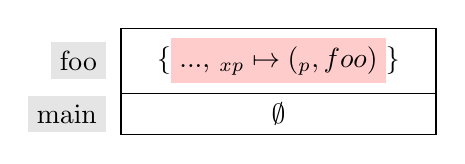
\begin{tikzpicture}[stack/.style={rectangle split, rectangle split parts=#1, draw, anchor=center, text centered},
        scope/.style={fill=gray!20, anchor=center}]
    \node[stack=2, minimum width=4.0cm] (s) {
    \nodepart{one} \{\colorbox{red!20}{..., $\Blockvar_{xp} \mapsto \onlyread{\set{(\Blockvar_p, \scope{foo})}}$}\}
    \nodepart{two} $\emptyset$
    };
    \node[scope, left=5pt of s.one west]   {\scope{foo}};
    \node[scope, left=5pt of s.two west]   {\scope{main}};
    \end{tikzpicture}   
}

\end{minipage}
\end{figure}


\end{frame}



\begin{frame}[fragile]
\frametitle{Nested restrict pointers (TLU)}
\begin{minted}[escapeinside=||,mathescape=true]{c}
// Scope $\scope{foo}$
int foo(int *restrict *restrict p, int *restrict *restrict q) {
    |\colorbox{red!20}{**p}| = 10;
    **q = 11;
    return **p;
}
\end{minted}

\vspace*{-2cm}

\begin{figure}[!h]
\begin{minipage}[t]{.36\textwidth}
\begin{minted}[escapeinside=||,mathescape=true]{c}
// Scope $\scope{main}$
int main() {
    int x;
    int* xp = &x;
    foo(&xp, &xp);
}
\end{minted}
\end{minipage}%
\begin{minipage}{.64\textwidth}

\executionannotation
{
\{ $\Blockvar_x \mapsto \vundef$, \\
    \ $\Blockvar_{xp} \mapsto \ptr{(\Blockvar_x, \emptyset)}$, \\
    \ $\Blockvar_p \mapsto \ptr{(\Blockvar_{xp}, \set{(\Blockvar_p, \scope{foo})})}$, \\
    \ $\Blockvar_q \mapsto \ptr{(\Blockvar_{xp}, \set{(\Blockvar_q, \scope{foo})})}$ \}
}
{
    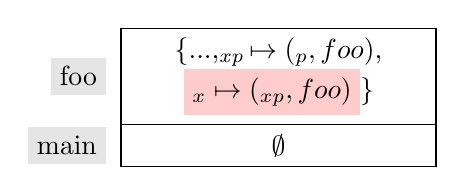
\begin{tikzpicture}[stack/.style={rectangle split, rectangle split parts=#1, draw, anchor=center, text centered},
        scope/.style={fill=gray!20, anchor=center}]
    \node[stack=2, minimum width=4.0cm] (s) {
    \nodepart[align=left]{one} \{$..., \Blockvar_{xp} \mapsto \onlyread{\set{(\Blockvar_p, \scope{foo})}}$, \\
                     \ \colorbox{red!20}{$\Blockvar_x \mapsto \restricted{\set{(\Blockvar_{xp}, \scope{foo})}}$}\}
    \nodepart{two} $\emptyset$
    };
    \node[scope, left=5pt of s.one west]   {\scope{foo}};
    \node[scope, left=5pt of s.two west]   {\scope{main}};
    \end{tikzpicture}   
}

\end{minipage}
\end{figure}

\end{frame}


\begin{frame}[fragile]
\frametitle{Nested restrict pointers (TLU)}

\begin{itemize}
    \item We now need to change the restrict state of $\Blockvar_{xp}$ to $\restrictedn$
    \item The only $\restrictedn$ state joinable with the current state is \colorbox{blue!20}{$\restricted{\set{(\Blockvar_p, \scope{foo})}}$}
    \item Problem: \textbf{not enough information} to produce this state, \ie the semantics did a store through $\ptr{(\Blockvar_x, \set{(\Blockvar_{xp}, \scope{foo})})}$
\end{itemize}

\leavevmode \\

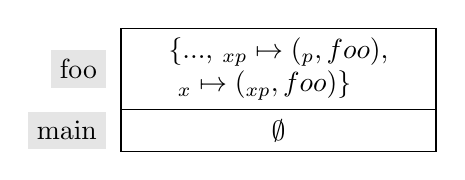
\begin{tikzpicture}[stack/.style={rectangle split, rectangle split parts=#1, draw, anchor=center, text centered},
    scope/.style={fill=gray!20, anchor=center}]
\node[stack=2, minimum width=4.0cm] (s) {
\nodepart[align=left]{one} \{..., $\Blockvar_{xp} \mapsto \onlyread{\set{(\Blockvar_p, \scope{foo})}}$, \\
                 \ $\Blockvar_x \mapsto \restricted{\set{(\Blockvar_{xp}, \scope{foo})}}$\}
\nodepart{two} $\emptyset$
};
\node[scope, left=5pt of s.one west]   {\scope{foo}};
\node[scope, left=5pt of s.two west]   {\scope{main}};
\end{tikzpicture}

\end{frame}


\begin{frame}
\frametitle{Nested restrict pointers (TLU)}

\begin{itemize}
    \item Idea: pointer value as a \textbf{tree} structure, to track how bases themselves are derived!
    \item $\ptr{(\Blockvar_x, \set{((\Blockvar_{xp}, \set{((\Blockvar_p, \emptyset), \scope{foo})}), \scope{foo})})}$ \\~\\
    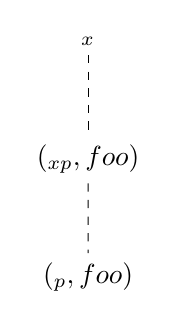
\begin{tikzpicture}[sibling distance=25mm,      edge from parent/.style={draw, dashed},
        every edge/.append style={->}    ]
    \node (root) {$\Blockvar_x$}
        child {node {$(\Blockvar_{xp}, \scope{foo})$}
        child {node {$(\Blockvar_p, \scope{foo})$}}
        };
    
    \end{tikzpicture}

\end{itemize}
    
\end{frame}



\begin{frame}[fragile]
\frametitle{Nested restrict pointers (TLU)}
\begin{minted}[escapeinside=||,mathescape=true]{c}
// Scope $\scope{foo}$
int foo(int *restrict *restrict p, int *restrict *restrict q) {
    |\colorbox{red!20}{**p}| = 10;
    **q = 11;
    return **p;
}
\end{minted}

\vspace*{-2cm}

\begin{figure}[!h]
\begin{minipage}[t]{.3\textwidth}
\begin{minted}[escapeinside=||,mathescape=true]{c}
// Scope $\scope{main}$
int main() {
    int x;
    int* xp = &x;
    foo(&xp, &xp);
}
\end{minted}
\end{minipage}%
\begin{minipage}{.7\textwidth}

\executionannotation
{
\{ $\Blockvar_x \mapsto \vundef$, \\
    \ $\Blockvar_{xp} \mapsto \ptr{(\Blockvar_x, \emptyset)}$, \\
    \ $\Blockvar_p \mapsto \ptr{(\Blockvar_{xp}, \set{((\Blockvar_p, \emptyset), \scope{foo})})}$, \\
    \ $\Blockvar_q \mapsto \ptr{(\Blockvar_{xp}, \set{((\Blockvar_q, \emptyset), \scope{foo})})}$ \}
}
{
    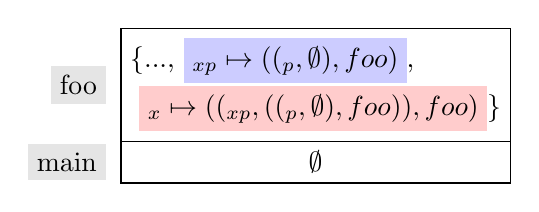
\begin{tikzpicture}[stack/.style={rectangle split, rectangle split parts=#1, draw, anchor=center, text centered},
        scope/.style={fill=gray!20, anchor=center}]
    \node[stack=2, minimum width=4.0cm] (s) {
    \nodepart[align=left]{one} \{..., \colorbox{blue!20}{$\Blockvar_{xp} \mapsto \restricted{\set{((\Blockvar_p, \emptyset), \scope{foo})}}$}, \\
                        \ \colorbox{red!20}{$\Blockvar_x \mapsto \restricted{\set{((\Blockvar_{xp}, \set{((\Blockvar_p, \emptyset), \scope{foo})}), \scope{foo})}}$}\}
    \nodepart{two} $\emptyset$
    };
    \node[scope, left=5pt of s.one west]   {\scope{foo}};
    \node[scope, left=5pt of s.two west]   {\scope{main}};
    \end{tikzpicture}   
}

\end{minipage}
\end{figure}

\end{frame}



\begin{frame}[fragile]
\frametitle{Nested restrict pointers (TLU)}
\begin{minted}[escapeinside=||,mathescape=true]{c}
// Scope $\scope{foo}$
int foo(int *restrict *restrict p, int *restrict *restrict q) {
    **p = 10;
    *|\colorbox{red!20}{*q}| = 11;
    return **p;
}
\end{minted}

\vspace*{-2cm}

\begin{figure}[!h]
\begin{minipage}[t]{.3\textwidth}
\begin{minted}[escapeinside=||,mathescape=true]{c}
// Scope $\scope{main}$
int main() {
    int x;
    int* xp = &x;
    foo(&xp, &xp);
}
\end{minted}
\end{minipage}%
\begin{minipage}{.7\textwidth}

\executionannotation
{
\{ $\Blockvar_x \mapsto \vundef$, \\
    \ $\Blockvar_{xp} \mapsto \ptr{(\Blockvar_x, \emptyset)}$, \\
    \ $\Blockvar_p \mapsto \ptr{(\Blockvar_{xp}, \set{((\Blockvar_p, \emptyset), \scope{foo})})}$, \\
    \ $\Blockvar_q \mapsto \ptr{(\Blockvar_{xp}, \set{((\Blockvar_q, \emptyset), \scope{foo})})}$ \}
}
{
    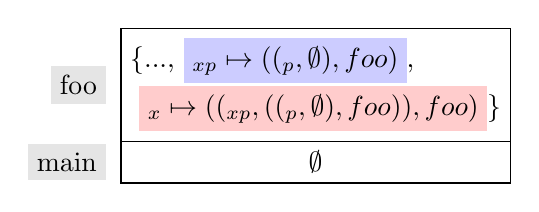
\begin{tikzpicture}[stack/.style={rectangle split, rectangle split parts=#1, draw, anchor=center, text centered},
        scope/.style={fill=gray!20, anchor=center}]
    \node[stack=2, minimum width=4.0cm] (s) {
    \nodepart[align=left]{one} \{..., \colorbox{blue!20}{$\Blockvar_{xp} \mapsto \restricted{\set{((\Blockvar_p, \emptyset), \scope{foo})}}$}, \\
                        \ \colorbox{red!20}{$\Blockvar_x \mapsto \restricted{\set{((\Blockvar_{xp}, \set{((\Blockvar_p, \emptyset), \scope{foo})}), \scope{foo})}}$}\}
    \nodepart{two} $\emptyset$
    };
    \node[scope, left=5pt of s.one west]   {\scope{foo}};
    \node[scope, left=5pt of s.two west]   {\scope{main}};
    \end{tikzpicture}   
}

\end{minipage}
\end{figure}

\end{frame}



\begin{frame}[fragile]
\frametitle{Nested restrict pointers (TLU)}
\begin{minted}[escapeinside=||,mathescape=true]{c}
// Scope $\scope{foo}$
int foo(int *restrict *restrict p, int *restrict *restrict q) {
    **p = 10;
    *|\colorbox{red!20}{*q}| = 11;
    return **p;
}
\end{minted}

\vspace*{-2cm}

\begin{figure}[!h]
\begin{minipage}[t]{.3\textwidth}
\begin{minted}[escapeinside=||,mathescape=true]{c}
// Scope $\scope{main}$
int main() {
    int x;
    int* xp = &x;
    foo(&xp, &xp);
}
\end{minted}
\end{minipage}%
\begin{minipage}{.7\textwidth}
\colorbox{red!20}{$\onlyread{\set{((\Blockvar_\text{\textcolor{blue}{$q$}}, \emptyset), \scope{foo})}} \joinsym  \restricted{\set{((\Blockvar_\text{\textcolor{blue}{$p$}}, \emptyset), \scope{foo})}} = ...$} \\

\executionannotation
{
\{ ..., \\
    \ $\Blockvar_q \mapsto \ptr{(\Blockvar_{xp}, \set{((\Blockvar_q, \emptyset), \scope{foo})})}$ \}
}
{
    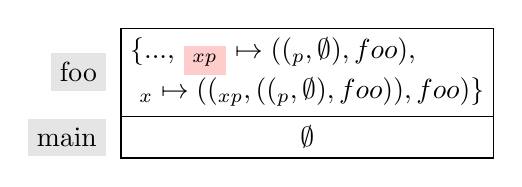
\begin{tikzpicture}[stack/.style={rectangle split, rectangle split parts=#1, draw, anchor=center, text centered},
        scope/.style={fill=gray!20, anchor=center}]
    \node[stack=2, minimum width=4.0cm] (s) {
    \nodepart[align=left]{one} \{..., \colorbox{red!20}{$\Blockvar_{xp}$} $\mapsto \restricted{\set{((\Blockvar_p, \emptyset), \scope{foo})}}$, \\
                        \ $\Blockvar_x \mapsto \restricted{\set{((\Blockvar_{xp}, \set{((\Blockvar_p, \emptyset), \scope{foo})}), \scope{foo})}}$\}
    \nodepart{two} $\emptyset$
    };
    \node[scope, left=5pt of s.one west]   {\scope{foo}};
    \node[scope, left=5pt of s.two west]   {\scope{main}};
    \end{tikzpicture}   
}

\end{minipage}
\end{figure}

\end{frame}






\begin{frame}[fragile]
\frametitle{Nested restrict pointers (TLU)}
\centering
\colorbox{red!20}{$\onlyread{\set{((\Blockvar_\text{\textcolor{blue}{$q$}}, \emptyset), \scope{foo})}} \joinsym  \restricted{\set{((\Blockvar_\text{\textcolor{blue}{$p$}}, \emptyset), \scope{foo})}} = \rsub$} \\

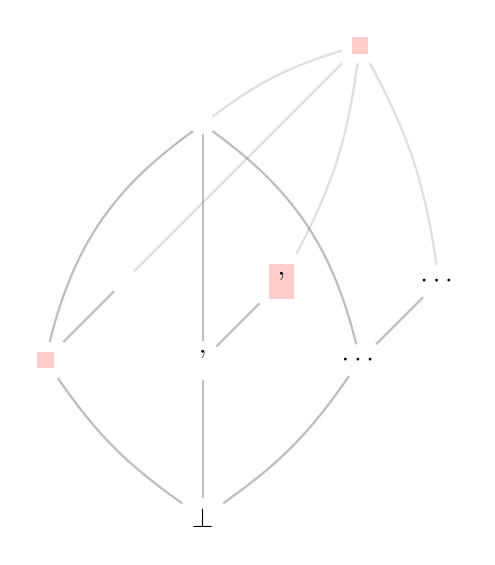
\begin{tikzpicture}
    \node (ub)     at (7,5) {\colorbox{red!20}{\rsub}};
    \node (un)     at (5,4) {\unresabbr};
    \node (rsbs)   at (4,2) {\resabbr{\Basesvar}};
    \node (rsbs')  at (6,2) {\colorbox{red!20}{\resabbr{\Basesvar'}}};
    \node (rsbs'') at (8,2) {$\cdots$};
    \node (orbs)   at (3,1) {\colorbox{red!20}{\orabbr{\Basesvar}}};
    \node (orbs')  at (5,1) {\orabbr{\Basesvar'}};
    \node (orbs'') at (7,1) {$\cdots$};
    \node (bot)    at (5,-1) {$\bot$};

    \path[thick, black, opacity=0.25]
    (bot) edge[bend left=10] node {} (orbs)
    (bot) edge node {} (orbs')
    (bot) edge[bend right=10] node {} (orbs'')
    
    (orbs) edge node {} (rsbs) 
    (orbs') edge node {} (rsbs')
    (orbs'') edge node {} (rsbs'')  
    
    (orbs) edge[bend left=20] node {} (un)
    (orbs') edge node {} (un)
    (orbs'') edge[bend right=20] node {} (un)

    (rsbs) edge[gray] node {} (ub)
    (rsbs') edge[bend right=10, gray] node {} (ub)
    (rsbs'') edge[bend right=10, gray] node {} (ub)

    (un) edge[bend left=10, gray] node {} (ub);
\end{tikzpicture}

\end{frame}


\begin{frame}[fragile]
\frametitle{Nested restrict pointers (TLU)}
\begin{itemize}
    \item Implemented a subtle subclause of the standard (in line with the GCC interpretation)
    \begin{itemize}    
        \item Updated pointer values to a \textbf{tree-like structure} to track how bases themselves are derived
    \end{itemize}
    \item Achieved our goal of giving undefined behavior \smiley{}
\end{itemize}

\end{frame}


\begin{frame}[fragile]
    \frametitle{Where are bases added to the pointer value?}

\begin{minted}[escapeinside=||,mathescape=true]{c}
// Scope $\scope{main}$
{
    int x; // $\&x = \Blockvar_x$
    int* restrict p = &x; // $\& \Blockvar_p$

    int* q = p; // Propagate the bases to q
    *p = ...;   // Used directly in lvalue position 
}
\end{minted}
{
\hspace*{-10pt}
\scriptsize
\begin{prooftree}
\AxiomC{$E(p) = \Blockvar_p$}
\RightLabel{\scriptsize{(EId)}}
\UnaryInfC{$\GEJudgment p, \Statevar \lval \colorbox{red!20}{$(\Blockvar_p, \emptyset)$}, \Statevar'$}

\AxiomC{$(\textcode{load} \ \Statevar' \ (\Blockvar_p, \emptyset)) = \ptr{(\Blockvar_x, \emptyset)}, \Statevar''$}

\AxiomC{$\isrestrict{e}$}

\RightLabel{\colorbox{red!20}{\scriptsize(ELvalConvRestrict)}}
\TrinaryInfC{$\GEJudgment p, \Statevar \rval \textcode{add\_prov} \ (\ptr{(\Blockvar_x, \emptyset)}) \ \colorbox{red!20}{$((\Blockvar_p, \emptyset), \scope{main})$}, \Statevar'' $}

% \RightLabel{\colorbox{red!20}{\scriptsize(Reduction)}}
% \UnaryInfC{$\GEJudgment p \rval \ptr{(\Blockvar_x, \set{((\Blockvar_p, \emptyset), \scope{main})})} $}

\RightLabel{\scriptsize(EDeref)}
\UnaryInfC{$\GEJudgment *p, \Statevar \lval (\Blockvar_x, \set{\colorbox{red!20}{$((\Blockvar_p, \emptyset), \scope{main})$}}), \Statevar''$}

\end{prooftree}
}
% \UnaryInfC{$p \lval l_1$}
% \AxiomC{$M(l_1) = \ptr{l_2}$}
% \RightLabel{\scriptsize(LValConv)}

% \BinaryInfC{$p \rval \ptr{l_2}$}
% \RightLabel{\scriptsize(EDeref)}

% \UnaryInfC{$*p \lval l_2$}
% \AxiomC{$M(l_2) = \ptr{l_3}$}
% \RightLabel{\scriptsize(LValConv)}

% \BinaryInfC{$\redm{*p \rval \ptr{l_3}}$}
% \RightLabel{\scriptsize(EDeref)}

% % \UnaryInfC{$\mathbin{**}p \lval l_3$}
% \end{prooftree}

\end{frame}





\end{document}
